%\usepackage{amsmath,amssymb,amsfonts}

% arara: makeindex: { style: class/ctuthesis }
% arara: bibtex

% The class takes all the key=value arguments that \ctusetup does,
% and a couple more: draft and oneside
\documentclass[twoside]{ctuthesis}

\ctusetup{
%	preprint = \today,% footer timestamp
%	mainlanguage = english,
%	titlelanguage = czech,
	mainlanguage = english,
	otherlanguages = {english},
	title-czech = {Metody numerického optimálního řízení pro minimalizaci času na kolo },
	title-english = {Numerical Optimal Control \\ for Minimum Lap Time },
	subtitle-czech = {Cesta do tajů kdovíčeho},
	%subtitle-english = {Journey to the who-knows-what wondeland},
	doctype = M,
	faculty = F3,
	%department-czech = {Katedra matematiky},
	%department-english = {Department of Control Engineering},
	author = {Bc. Richard Ciglanský},
	supervisor = {doc. Ing. Zdeněk Hurák, Ph.D.},
	%supervisor-address = {Ústav X, \\ Uliční 5, \\ Praha 99},
	%supervisor-specialist = {John Doe},
	%fieldofstudy-english = {Control engineering},
	%subfieldofstudy-english = {Mathematical Modelling},
	%fieldofstudy-czech = {Matematcké inženýrství},
	%subfieldofstudy-czech = {Matematické modelování},
	keywords-czech = {NLP, simulace času na kolo, optimální řízení, IPOPT, vozidlová dynamika, kolokační metody, Julia, citlivostní analýza},
	keywords-english = {NLP,optimization, automatic differentiation, twin-track model, pacejka, julia, scalability, Ipopt, MadNLP, MUMPS, ma97, CuDSS, sensitivty analysis},
	day = 22,
	month = 5,
	year = 2026,
%	specification-file = {ctutest-zadani.pdf},
%	front-specification = true,
%	front-list-of-figures = false,
%	front-list-of-tables = false,
%	monochrome = true,
%	layout-short = true,
}

\ctuprocess

\addto\ctucaptionsczech{%
	\def\supervisorname{Vedoucí}%
	\def\subfieldofstudyname{Studijní program}%
}

\ctutemplateset{maketitle twocolumn default}{
	\begin{twocolumnfrontmatterpage}
		%\ctutemplate{twocolumn.thanks}
		%\ctutemplate{twocolumn.declaration}
		\ctutemplate{twocolumn.abstract.in.titlelanguage}
		\ctutemplate{twocolumn.abstract.in.secondlanguage}
		\ctutemplate{twocolumn.tableofcontents}
		\ctutemplate{twocolumn.listoffigures}
	\end{twocolumnfrontmatterpage}
}

% Theorem declarations, this is the reasonable default, anybody can do what they wish.
% If you prefer theorems in italics rather than slanted, use \theoremstyle{plainit}
\theoremstyle{plain}
\newtheorem{theorem}{Theorem}[chapter]
\newtheorem{corollary}[theorem]{Corollary}
\newtheorem{lemma}[theorem]{Lemma}
\newtheorem{proposition}[theorem]{Proposition}

\theoremstyle{definition}
\newtheorem{definition}[theorem]{Definition}
\newtheorem{example}[theorem]{Example}
\newtheorem{conjecture}[theorem]{Conjecture}

\theoremstyle{note}
\newtheorem*{remark*}{Remark}
\newtheorem{remark}[theorem]{Remark}

% Abstract in Czech
\begin{abstract-czech}
Táto práca skúma a implementuje metódy riešenia problému minimálneho času manévrovania (simulácia času na kolo) pre cestné vozidlá. Problém je rozdelený na menšie podproblémy, pre ktoré už existujú vyspelé softvérové nástroje. Týmito podproblémami sú: modelovanie pretekárskeho vozidla, transkripcia úlohy optimálneho riadenia na úlohu nelineárneho programovania (NLP), riešenie NLP, riešenie sústav lineárnych rovníc a citlivostná analýza. Každý podproblém je skúmaný v kontexte dynamiky vozidla a je predstavená implementácia v jazyku Julia postavená na knižnici JuMP . Implementácia podporuje viacero kolokačných schém Gauss Legendre, Radau a Lobatto spolu s adaptívnym zjemňovaním siete. Rôzne modely vozidiel rastúcej zložitosti, stratégie transkripcie a backendy lineárnych riešičov (MUMPS, HSL MA57/MA97) sú porovnané na reprezentatívnych okruhoch a je analyzovaná parametrická citlivosť optimálneho času na kolo.

\end{abstract-czech}

% Abstract in English
\begin{abstract-english}
The thesis researches and implements ways of solving the minimum-time maneuvering problem (lap-time simulation) for road vehicles. It divides the problem into smaller subproblems for which mature software methods already exist. The subproblems are: race-car modeling, transcription of the optimal control problem into an NLP, solving the NLP, solving sets of linear equations, and sensitivity analysis. Each subproblem is examined in the context of vehicle dynamics, and a Julia-based implementation built on JuMP and Ipopt is presented. The framework supports several collocation schemes (Gauss-Legendre, Radau, and Lobatto) together with adaptive mesh refinement. Various vehicle models of increasing complexity, transcription strategies, and linear solver backends (MUMPS, HSL MA57/MA97) are benchmarked on representative circuits, and the parametric sensitivity of the optimal lap time is analyzed.

\end{abstract-english}

% Acknowledgements / Podekovani
\begin{thanks}
Děkuji ČVUT, že mi je tak dobrou \emph{alma mater}.
\end{thanks}

% Declaration / Prohlaseni
\begin{declaration}
Prohlašuji, že jsem předloženou práci vypracoval samostatně, a že jsem uvedl veškerou použitou literaturu.
V Praze, \ctufield{day}.~\monthinlanguage{title}~\ctufield{year}
%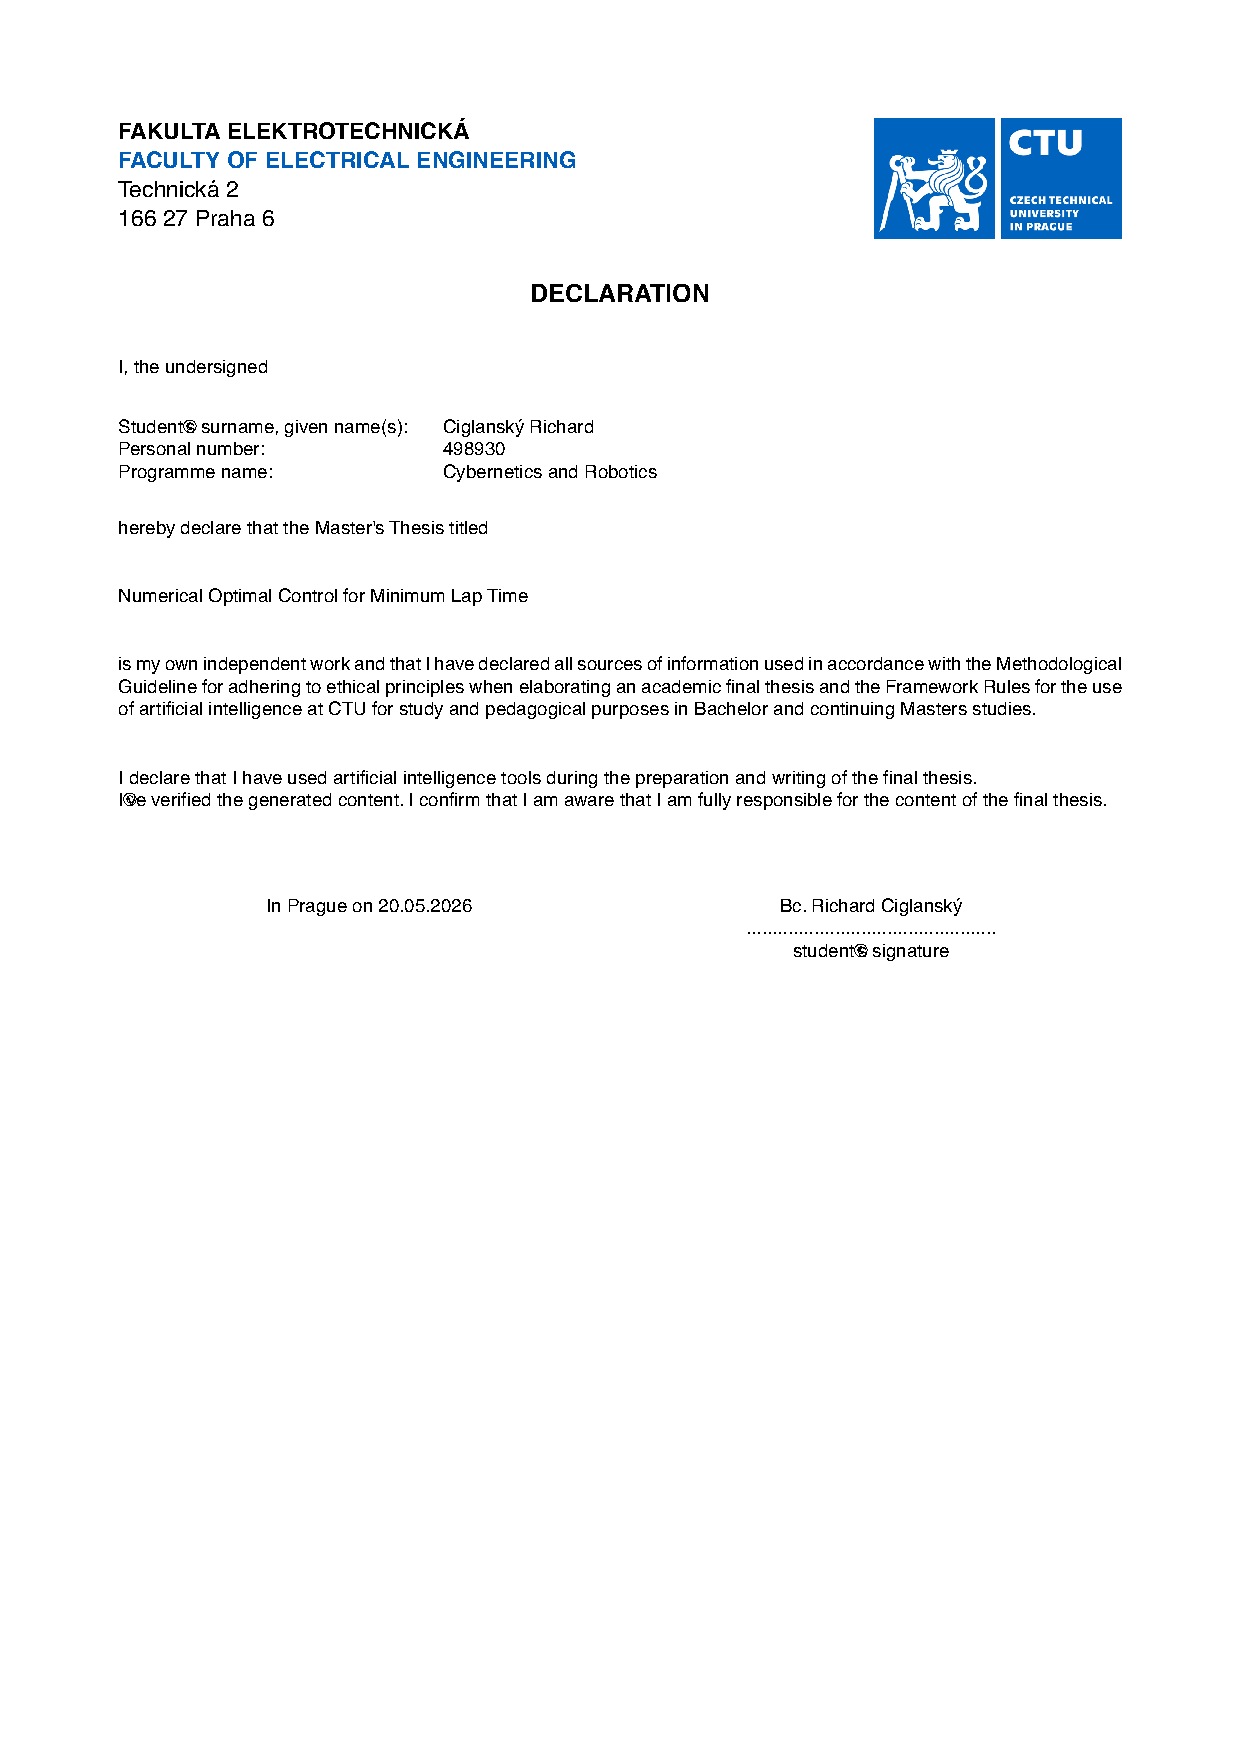
\includepdf[pages=-]{../sync/document_24_filename.pdf}


\end{declaration}

% Only for testing purposes
\listfiles
\usepackage{lmodern}
\usepackage[pagewise]{lineno}
\usepackage{lipsum,blindtext}
\usepackage{mathrsfs} % provides \mathscr used in the ridiculous examples
\usepackage{bm}
\usepackage{longtable}
\usepackage{tikz}
\usepackage{emoji}
\usepackage{fontspec}
\usetikzlibrary{positioning,calc,shapes.geometric,arrows.meta,backgrounds,babel}
\usepackage{subcaption}

\begin{document}

\maketitle

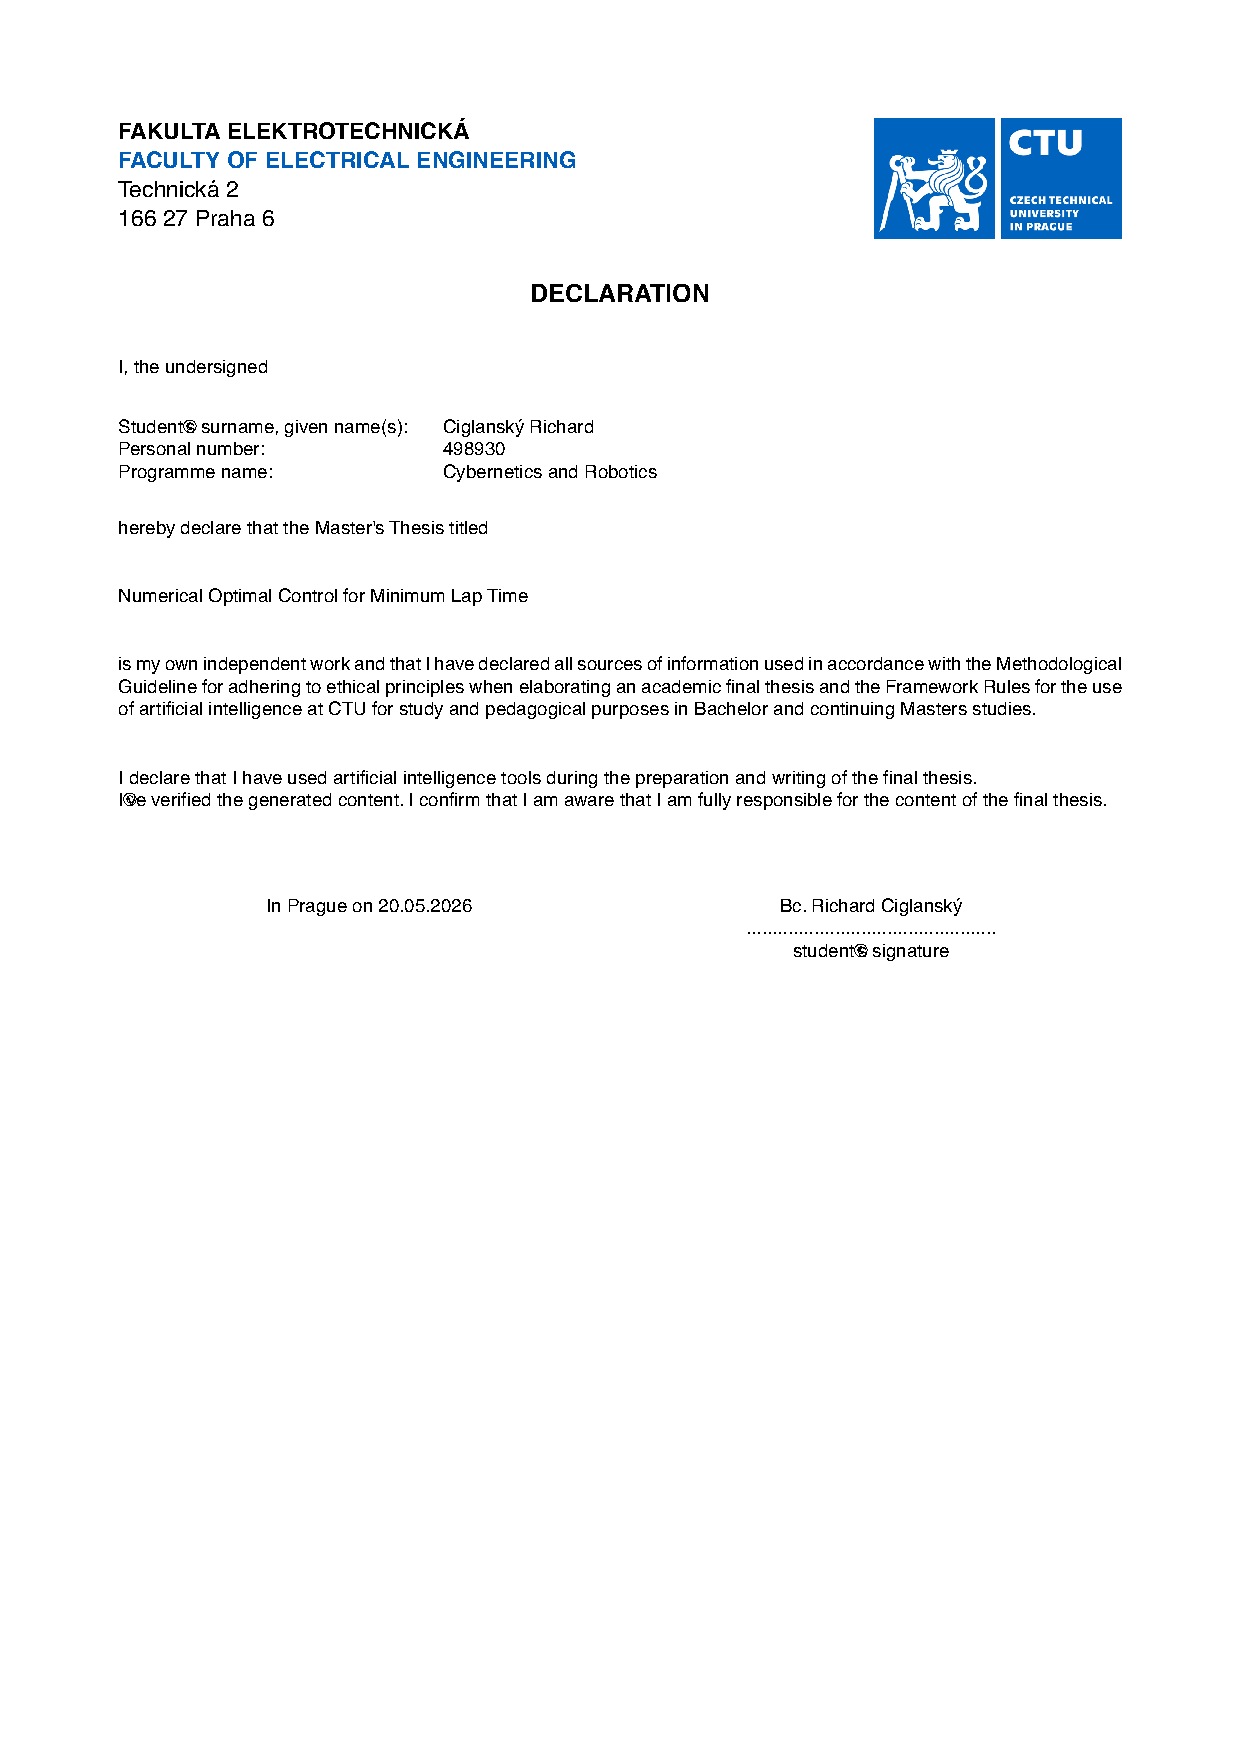
\includepdf[pages=-]{../sync/document_24_filename.pdf}

\chapter{Introduction}
\section{Motivation}
Topic of this thesis is motivated, by my work in Formula Student team eForce
Prague Formula, where I worked on real-time vehicle dynamics control software.
There I got intricately exposed to problems faced by racing teams, such as
should we increase the aerodynamic downforce at the cost of higher drag? Should
we put accumulator in the middle of vehicle, to decrease moment of inertia?
Should the aerodynamics be designed for straight line drive, or for steady
state turning? How to use limited energy from accumulator more effectively, how
faster can we go if we made better power limiting algorithm? How large the
accumulator should be? Which torque allocation algorithm should be used? How to
design the suspension kinematics to maximize the tire utilization? Is rear
wheel steering worth the increased weight? All of these problems can be
analyzed by using purpose built tool, good engineering practices or using pen
and paper with heavily simplified model. Formula student season is 10 months
for development and construction of the vehicle, 2 months for competition. That
puts enormous pressure on deciding on vehicle concept fast. In my opinion what
formula student teams need is a tool to quickly evaluate different car
concepts. As my bachelor thesis I created a prototype of such tool, goals of
this thesis come from computational and user experience form my previous tool.

\section{Goals}
\begin{itemize}
	\item Primary goal of this thesis is to investigate available methods for numerical
	      optimal control with respect to their suitability for planning an optimal
	      trajectory of a vehicle aiming to achieve the minimum lap time on a racing
	      circuit. To do this for various vehicle concepts, thesis has to present a
	      vehicle modelling framework.
	\item Benchmark performance of available numerical methods
	\item Thesis should present a tool for convenient vehicle modelling, and vehicle
	      concept evaluation.
	\item Support vehicle parameter optimization, using any vehicle parameter as control
	      input and sensitivity analysis of vehicle parameters.
	\item Goal is not precise vehicle modeling and validation, goal is to create a
	      framework to perform vehicle concept analyses easily.
\end{itemize}

%Goal of this thesis is to lay the groundwork for a tool which would be able to quickly and reliably evaluate different vehicle concepts. 
%Thesis should presenta framework for simulating multiple complexities of vehicle model. 
%like in bachelor thesis where i preformeda nd vladiated analysis on vehicle components, 

%Each parameter can be static, desgin varaible, or control variable.

%For fast and sufficiently accurate vehicle simulation it is crucial to explore and compare
%various methods of transcribing the optimal control problem

% such as global collocation using a single polynomial over the whole horizon, multi-segment collocation that splits the horizon into smaller intervals each with its own polynomial, and Runge Kutta methods.

%Goal is not to present results of specific car model or recommendation on car
%design, therefore validation and verification were not done in this thesis. i
%ahev already done them in bachelor thesis
%\cite{ciglanskyAnalysisVehicleComponents}

\section{Structure of thesis}
First part of thesis with vehicle modelling in the context of optimal control.
A universal model structure inspired by \cite{brown_engineering_2006} is
presented. Then the theory of optimal control idem spat ja neviem co pisat uz.
\begin{enumerate}
	\item ODE models of cars
	\item Solving methods: time marching forward, backward pass, NLP,
	\item Collocation (p, h, hp refinement), integral + differential form (Gauss-Radau,
	      Legendre, Lobatto)
	\item Implementation overview, Algorithmic differentiation, JUMP/Examples/InfiniteOpt
	      + Julia, Python/MATLAB, CasADi, interior point solvers
	\item Actual implementation and results
	\item Conclusion
\end{enumerate}

\section{Literature overview/ survey of laptime simulators}


Lap-time prediction dates back to the 1950s. Computers became common in the
1970s and quasi-steady-state (QSS) methods became the standard approach for
MLTS.\@ QSS is still what most race engineers mean by ``lap-time simulation''.
In QSS the vehicle is a point mass on a fixed racing line, with lateral and
longitudinal accelerations bounded by a steady-state performance
envelope~\cite{Roland1971}. Transient effects such as yaw acceleration are
ignored. MLTS was first formulated as an optimal control problem in the late
1980s~\cite{Hatwal1986SomeIS}. A survey of current methods is given
in~\cite{massaroMinimumlaptimeOptimisationSimulation2021}. The work of Perantoni
and Limebeer~\cite{perantoniOptimalControlFormula2014} is the main reference:
it uses a track-fixed coordinate system, switches the independent variable from
time to travelled distance, and applies the formulation to a twin-track
Formula 1 model with some vehicle parameters as decision variables. Parts of
this thesis build on it. MLTS is still an active research area because better
predictions give measurable setup gains, but higher fidelity models cost more
solver time. The authors of~\cite{ComputationallyEfficientFramework} use
sequential convex programming to cut compute cost without losing accuracy.

A very popular laptime simulator is OptimumLap from OptimumG
\cite{OptimumLapOptimumG}, It is a free commercial tool advertised to achieve
10\% accuracy with real vehicles. It uses Quasi Steady State methods (QSS) This
is the standard tool for laptime simulations. Open source implementation of the
same method \cite{mc12027Mc12027OpenLAPLapTimeSimulator2026}, My implementation of this method in chapter ??. QSS methods are very fast, but the models for which they can be used is equally very simple.

Popular open source C++ implementation of laptime simulator using nonlinear
programming and automatic differentiaoton\cite{manzaneroJuanmanzaneroFastestlap2026}. It uses IPOPT and
CppAD\cite{CoinorCppAD2026}. Vehicle model is 6DOF twintrack. Other implementations are
work from austria or germany\cite{Heilmeier2019} class project from Georgia institute of technology \cite{2026ClassProject}


\part{Theory}
\chapter{Vehicle and Track modeling framework}
The goal of the thesis is to select a sufficiently accurate yet computationally tractable model of the vehicle.
There is no single vehicle model that fits all requirements of race engineers. For each problem, a different complexity of the vehicle model is sufficient, e.g.\ for analysis of a power-limit algorithm, the lateral dynamics of the vehicle can be heavily simplified, and simple transcription and solving methods yield sufficient accuracy within a fraction of a second. This is described in Section~\ref{QSS}. Whereas analysis of the torque allocation problem requires the full twin-track model and more computationally expensive transcription and solving methods. Therefore, a vehicle modeling framework is needed to satisfy the needs of different types of analyses.

\section{Graph-centered approach for vehicle modeling}
The structure of the vehicle model has to allow extending or changing components, so that different vehicle concepts can be simulated with minimal coding. The book~\cite{brown_engineering_2006} describes a modeling framework that allows creating car components as modules with a flow and effort interface. This common interface heavily simplifies the process of creating a car model, as modules can be reused and chained together easily.
The vehicle components are: chassis, wheel pivot, tire, aerodynamics, suspension, motor, and accumulator.

\begin{figure}[H]
	\centering
	\begin{tikzpicture}[
			box/.style={rectangle, draw, thick, minimum width=3cm, minimum height=2.5cm, align=center},
			arr/.style={->, thick}
		]

		\node[box] (wa) {Wheel\\Pivot};

		% Top-left input: omega, v
		\draw[arr] (-3.5, 0.5) -- node[above] {$\symbf{\omega},\, \symbf{v}$} ($(wa.west)+(0,0.5)$);

		% Top-right output: v_tire
		\draw[arr] ($(wa.east)+(0,0.5)$) -- node[above] {$\symbf{v}_{tire}$} (3.5, 0.5);

		% Bottom-left output: F_CoG, M_CoG
		\draw[arr] ($(wa.west)+(0,-0.5)$) -- node[below] {$\symbf{F}_{CoG},\, \symbf{M}_{CoG}$} (-4.5, -0.5);

		% Bottom-right input: F_tire
		\draw[arr] (3.5, -0.5) -- node[below] {$\symbf{F}_{tire}$} ($(wa.east)+(0,-0.5)$);

	\end{tikzpicture}
	\caption{Wheel Pivot}
	\label{fig:wheel_pivot}
\end{figure}



\section{Tire-road interface modeling}
The role of the tire model in this thesis is to calculate forces acting on the tire from the relative velocity and angle between tire and road. The input of a general tire model is 3 velocities and 3 angles, and the output is 3 forces.\label{tiremodel}


\begin{figure}[H]
	\centering
	\begin{tikzpicture}[
			box/.style={rectangle, draw, thick, minimum width=3cm, minimum height=2.5cm, align=center},
			arr/.style={->, thick}
		]

		\node[box] (tire) {Tire};

		% Left-top input: tire-frame velocity vector
		\draw[arr] (-4, 0.5) -- node[above] {$\symbf{v}_{tire}$} ($(tire.west)+(0,0.5)$);

		% Left-bottom input: drive/brake torque
		\draw[arr] (-4, -0.5) -- node[below] {$T_{in}$} ($(tire.west)+(0,-0.5)$);

		% Top input: normal force from suspension
		\draw[arr] (0, 2) -- node[right] {$F_z$} (tire.north);

		% Output bends around the right side and returns to the left (back to wheel pivot)
		\draw[arr] ($(tire.east)+(0,-0.5)$) -- (3, -0.5) -- (3, -2.2) -- node[below] {$\symbf{F}_{tire}$} (-4, -2.2);

	\end{tikzpicture}
	\caption{Tire component}\label{fig:tire}
\end{figure}


Most forces that govern vehicle movement are transferred by the tires. The tire is considered to be the most important system of a vehicle and it is notoriously difficult to model~\cite{Yuki-2019}. Thus tires need to be modeled carefully. Not only are there many parameters, such as tire wear, tire temperature, road roughness, road wetness, tire pressure, etc., that affect the resultant forces, but they are also constantly changing during the lap. Therefore they are difficult to measure and model precisely. This paragraph is adapted from my bachelor thesis~\cite{ciglanskyAnalysisVehicleComponents}.
Implementation of specific models is covered in Part~III, Implementation.


\subsection{Linear tire}
\label{linearTire}
This tire model maps lateral slip angle
\begin{equation}
    \alpha = -\arctan\!\left(\frac{v_y}{v_x}\right),
    \label{eq:slip_angle}
\end{equation}
into lateral force
\begin{equation}
    F_y = \frac{\alpha}{\alpha_\text{max}}\,\mu\,F_z.
    \label{eq:linear_tire_lat}
\end{equation}
The tire model does not consider spinning of the wheels. Therefore, there is no longitudinal slip, and the motor force acts directly on the wheel pivot point.
\begin{equation}
    F_x = \frac{T_\text{wheel}}{R} + F_\text{brake}.
    \label{eq:linear_tire_lon}
\end{equation}
Forces are constrained by friction ellipse
\begin{equation}
    F_x^2 + F_y^2 \;\leq\; (\mu F_z)^2.
    \label{eq:friction_circle}
\end{equation}

The implication of neglecting tire spinning is that energy from the motor is not used to spin up the wheels and goes entirely into accelerating the car, creating a large discrepancy from how a real vehicle operates. In this and the following models this effect is not accounted for.
\subsection{Magic Formula tire}
The Magic Formula tire model, developed by Hans B. Pacejka~\cite{pacejka}, is an empirically derived formula that describes tire forces. The full Magic Formula model has around 80 parameters and many variants. The variant described here was taken from~\cite{2026ClassProject} and has only 6 parameters.\label{pacejka}
\begin{equation}
    \alpha = -\arctan\!\left(\frac{v_y}{v_x}\right).
    \label{eq:pac_slip}
\end{equation}
Parameter $D$ is the peak factor
\begin{equation}
    D = \mu\, F_z \left(1 - \epsilon\, \frac{F_z}{F_{z,\text{ref}}}\right),
    %\qquad \beta = 0.0813,\ F_{z,\text{ref}} = 3000~\text{N}
    \label{eq:pac_peak}
\end{equation}
$\epsilon$ models degressive behavior, the peak lateral force of a real tire does not grow linearly with normal force. $F_{z,\text{ref}}$ is the nominal normal tire load~\cite{2026ClassProject}. The lateral force is then computed according to the Magic Formula from~\cite{pacejka},
\begin{equation}
    F_y = D \sin\!\Big( C \arctan\!\big( B\alpha - E\,(B\alpha - \arctan(B\alpha)) \big) \Big),
    \label{eq:pac_fy}
\end{equation}
where $C$ is the shape factor, $B$ is the stiffness factor and $E$ is the curvature factor. These parameters are fitted to real tire measurement data.
Then tire rolling resistance $C_r$ is added and the friction ellipse is the same as for the linear tire,
\begin{equation}
    F_x = \frac{T_\text{wheel}}{R} + F_\text{brake} + C_r\, F_z,
    \label{eq:pac_fx}
\end{equation}

\begin{equation}
    \left(\frac{F_x}{\mu F_z}\right)^{\!2} + \left(\frac{F_y}{\mu F_z}\right)^{\!2} \;\leq\; 1.
    \label{eq:pac_friction_circle}
\end{equation}

%\subsection{Linear tire}
%Simplest tire model. Tire is defined by friction ellipse and an angle at which
%the slip angle is highest
%\subsection{Pacejka}
%Pacejka tire uses
%\subsection{Extended Pacejka}
\section{Chassis model}
The chassis is modeled as a point mass located at the center of gravity (CoG), carrying the full vehicle mass and yaw inertia, with the wheel pivot points defined relative to it. The chassis model is responsible for computing the state-derivative vector from all forces and moments acting on the CoG. Equations~\ref{cogeq1}--\ref{coeq2} describe the computation.
\begin{table}[!ht]
	\centering
	\begin{tabular}{lll}
		\hline
		\textbf{Symbol} & \textbf{Unit}     & \textbf{Description}                            \\
		\hline
		$m$             & kg          & Mass       \\
		$I_z$           & $kg \cdot m^2$               & Yaw Inertia                               \\
		$w$             & m & Width of vehicle \\
		\hline
	\end{tabular}
	\caption{Parameters of the chassis model.}
	\label{tab:chassis-params}
\end{table}

\begin{equation}
    \symbf{M}_{\!CoG,i} = \symbf{r}_i \times \symbf{F}_i, \qquad
    \symbf{F}_i = \begin{bmatrix} F_{x_i} \\ F_{y_i} \\ 0 \end{bmatrix}.
    \label{cogeq1}
\end{equation}
\begin{equation}
    \symbf{F}_{\!CoG} = \sum_i \symbf{F}_i + \begin{bmatrix} F_\text{drag} \\ 0 \\ 0 \end{bmatrix}, \qquad
    \symbf{M}_{\!CoG} = \sum_i \symbf{M}_{\!CoG,i}.
\end{equation}
\begin{equation}
    \dot{\symbf{v}} = \frac{\symbf{F}_{\!CoG}}{m} - \symbf{\omega} \times \symbf{v}, \qquad
    \dot{\symbf{\omega}} = \frac{\symbf{M}_{\!CoG}}{I}.
\end{equation}
\begin{equation}
    \symbf{x} = \begin{bmatrix} v_x \\ v_y \\ \psi \\ \dot{\psi} \end{bmatrix}, \qquad
    \dot{\symbf{x}} = \begin{bmatrix} \dot{v}_x \\ \dot{v}_y \\ \dot{\psi} \\ \ddot{\psi} \end{bmatrix}.
    \label{coeq2}
\end{equation}
The chassis also imposes a constraint on the location on the track to prevent the vehicle from leaving it.


\section{Wheel Pivot model}
The wheel pivot point is modeled as a transformer. It defines the transformation of CoG velocities into the tire frame and then transforms tire forces and torque into the pivot frame. The angular velocity and position vectors are formed from the yaw rate $\dot{\psi}$, the longitudinal distance $l_i$ of the axle from the center of gravity, and the lateral distance $\pm b/2$ of the wheel from the vehicle centerline:
\begin{equation}
    \symbf{\omega} = \begin{bmatrix} 0 \\ 0 \\ \dot{\psi} \end{bmatrix}, \qquad
    \symbf{r}_i    = \begin{bmatrix} l_i \\ b/2 \\ 0 \end{bmatrix},
\end{equation}
where $b$ is the track width. Velocity at each tire pivot point is:
\begin{equation}
    \symbf{v}_{p_i} = \symbf{v} + \symbf{\omega} \times \symbf{r}_i.
\end{equation}
Velocities are then rotated from the pivot frame into the tire frame using the
steering angle $\delta_i$:
\begin{equation}
    R_t = \begin{bmatrix}
        \cos\delta_i & -\sin\delta_i & 0 \\
        \sin\delta_i &  \cos\delta_i & 0 \\
        0            &  0            & 1
    \end{bmatrix}, \qquad
    \symbf{v}_{t_i} = R_t\,\symbf{v}_{p_i}.
\end{equation}
Tire forces $F_{tx}$ and $F_{ty}$ are computed from $\symbf{v}_{t_i}$ by the tire
model. Forces are then rotated back to the pivot frame:
\begin{equation}
    \begin{bmatrix} F_{x_i} \\ F_{y_i} \end{bmatrix}
    =
    \begin{bmatrix}
         \cos\delta_i & \sin\delta_i \\
        -\sin\delta_i & \cos\delta_i
    \end{bmatrix}
    \begin{bmatrix} F_{tx} \\ F_{ty} \end{bmatrix}.
\end{equation}

\begin{figure}[H]
    \centering
    \begin{tikzpicture}[
            box/.style={rectangle, draw, thick, minimum width=3.5cm, minimum height=3cm, align=center},
            arr/.style={->, thick}
        ]

        \node[box] (wa) {Wheel\\Pivot};

        % Top input: steering angle delta_i (control)
        \draw[arr] (0, 2.2) -- node[right] {$\delta_i$} (wa.north);

        % Left-top input: CoG velocity and angular velocity
        \draw[arr] (-4.5, 0.6) -- node[above] {$\symbf{v},\,\symbf{\omega}$} ($(wa.west)+(0,0.6)$);

        % Left-bottom output: forces and moment on CoG
        \draw[arr] ($(wa.west)+(0,-0.6)$) -- node[below] {$\symbf{F}_{\!CoG},\,\symbf{M}_{\!CoG}$} (-4.5, -0.6);

        % Right-top output: tire-frame velocity to tire model
        \draw[arr] ($(wa.east)+(0,0.6)$) -- node[above] {$\symbf{v}_{t_i}$} (4.5, 0.6);

        % Right-bottom input: tire forces from tire model
        \draw[arr] (4.5, -0.6) -- node[below] {$\symbf{F}_{tire}$} ($(wa.east)+(0,-0.6)$);

    \end{tikzpicture}
    \caption{Wheel Pivot component}\label{fig:wheel_pivot_io}
\end{figure}

\section{Aerodynamics model}
The aerodynamic model is treated as a nonlinear resistance element, mapping velocity into forces. Drag and down-force scale with the square of longitudinal velocity:
\begin{equation}
	F_\text{drag} = \tfrac{1}{2}\,\rho\,C_D\,v_x^2, \qquad
	F_\text{lift} = \tfrac{1}{2}\,\rho\,C_L\,v_x^2.
\end{equation}
The down-force is split between front and rear axles by the center of pressure
ratio $\mathrm{CoP} \in [0,1]$, where $\mathrm{CoP}=0.5$ corresponds to a balanced
distribution. Air density $\rho$ is taken as $1.225\,\mathrm{kg/m^3}$ at sea
level. Coefficients $C_L$, $C_D$ and $\mathrm{CoP}$ used per vehicle model are
listed in Table~\ref{tab:aero-params}.

\begin{table}[!ht]
	\centering
	\begin{tabular}{lll}
		\hline
		\textbf{Symbol} & \textbf{Unit}     & \textbf{Description}                            \\
		\hline
		$C_L$           & ---               & Lift coefficient (negative = down-force)         \\
		$C_D$           & ---               & Drag coefficient                                \\
		$\mathrm{CoP}$  & ---               & Center of pressure (front axle share, $0$--$1$) \\
		$\rho$          & $\mathrm{kg/m^3}$ & Air density                                     \\
		\hline
	\end{tabular}
	\caption{Parameters of the aerodynamic model.}
	\label{tab:aero-params}
\end{table}

\begin{figure}[H]
    \centering
    \begin{tikzpicture}[
            box/.style={rectangle, draw, thick, minimum width=3.5cm, minimum height=2.5cm, align=center},
            arr/.style={->, thick}
        ]

        \node[box] (aero) {Aerodynamics};

        % Left input: longitudinal velocity
        \draw[arr] (-4, 0) -- node[above] {$v_x$} (aero.west);

        % Right-top output: drag force
        \draw[arr] ($(aero.east)+(0,0.5)$) -- node[above] {$F_\text{drag}$} (4, 0.5);

        % Right-bottom output: downforce
        \draw[arr] ($(aero.east)+(0,-0.5)$) -- node[below] {$F_\text{down}$} (4, -0.5);

    \end{tikzpicture}
    \caption{Aerodynamics component}\label{fig:aero}
\end{figure}

This model is sufficient when the vehicle is driving relatively straight, i.e.\ when lateral acceleration is roughly zero. With high lateral acceleration this model is no longer valid, because air speeds differ on the left and right side of the car and the car also starts rolling, one side of the vehicle is closer to the ground than the other, creating an imbalance of lift forces.

\section{Suspension model}
The purpose of the suspension in a car is to maintain tire contact, distribute the load from lateral load transfer to better utilize the tires, and use kinematics to make use of camber thrust. Commonly the suspension of a car consists of springs, dampers and the mounting with tie rods. In this thesis, the suspension model had to be significantly simplified. Modeling each wheel with a damper, spring and its own kinematics is beyond the scope of this thesis. However, the model structure allows for it, but I did not have enough time to implement it. Such a model would be very beneficial toward the goal of scalability. Without it, the model scalability is limited, as dividing force between more than two wheels on an axle is a statically indeterminate problem.
\begin{figure}[H]
    \centering
    \begin{tikzpicture}[
            box/.style={rectangle, draw, thick, minimum width=3.8cm, minimum height=3.6cm, align=center},
            arr/.style={->, thick}
        ]

        \node[box] (sus) {Suspension};

        % Left-top input: downforce
        \draw[arr] (-4.5, 0.9) -- node[above] {$F_\text{down}$} ($(sus.west)+(0,0.9)$);

        % Left-middle input: center of pressure
        \draw[arr] (-4.5, 0.0) -- node[above] {$\mathrm{CoP}$} ($(sus.west)+(0,0.0)$);

        % Left-bottom input: chassis (mass + CoG offsets)
        \draw[arr] (-4.5, -0.9) -- node[below] {$m,\,x_{CoG},\,y_{CoG}$} ($(sus.west)+(0,-0.9)$);

        % Right outputs: four wheel normal loads
        \draw[arr] ($(sus.east)+(0, 1.2)$) -- node[above] {$F_{z,FL}$} (4.5,  1.2);
        \draw[arr] ($(sus.east)+(0, 0.4)$) -- node[above] {$F_{z,FR}$} (4.5,  0.4);
        \draw[arr] ($(sus.east)+(0,-0.4)$) -- node[below] {$F_{z,RL}$} (4.5, -0.4);
        \draw[arr] ($(sus.east)+(0,-1.2)$) -- node[below] {$F_{z,RR}$} (4.5, -1.2);

    \end{tikzpicture}
    \caption{Suspension component}\label{fig:suspension}
\end{figure}
Two suspension variants are used in this thesis: static distribution and dynamic distribution.

\subsection{Static suspension}
\label{staticsusp}
The static suspension distributes the vehicle's mass and the force from aerodynamics according to the position of the center of gravity and the center of pressure. This trivial implementation is possible only for two axles, three or more axles would make this a statically indeterminate system.
\begin{equation}
    \begin{aligned}
        F_{z,FL} &= \bigl(m g\, x_\text{CoG} + F_\text{lift}\,\text{CoP}\bigr)(1 - y_\text{CoG}) \\
        F_{z,FR} &= \bigl(m g\, x_\text{CoG} + F_\text{lift}\,\text{CoP}\bigr)\, y_\text{CoG}     \\
        F_{z,RL} &= \bigl(m g\,(1-x_\text{CoG}) + F_\text{lift}(1-\text{CoP})\bigr)(1 - y_\text{CoG}) \\
        F_{z,RR} &= \bigl(m g\,(1-x_\text{CoG}) + F_\text{lift}(1-\text{CoP})\bigr)\, y_\text{CoG}
    \end{aligned}
\end{equation}
\subsection{Dynamic suspension}
This suspension variant takes into account the load transfer caused by longitudinal and lateral accelerations. It is adapted from~\cite{2026ClassProject}.
\begin{equation}
    \begin{aligned}
        F_{z,FL} &= \!\left(m g\, x_\text{CoG} - \frac{m\, a_x h_\text{CoG}}{L}\right)\!(1-y_\text{CoG})
                  + \tfrac{1}{2} F_\text{down}\,\text{CoP} - \tfrac{1}{2}\Delta F_y \\[3pt]
        F_{z,FR} &= \!\left(m g\, x_\text{CoG} - \frac{m\, a_x h_\text{CoG}}{L}\right)\! y_\text{CoG}
                  + \tfrac{1}{2} F_\text{down}\,\text{CoP} + \tfrac{1}{2}\Delta F_y \\[3pt]
        F_{z,RL} &= \!\left(m g\,(1-x_\text{CoG}) + \frac{m\, a_x h_\text{CoG}}{L}\right)\!(1-y_\text{CoG})
                  + \tfrac{1}{2} F_\text{down}\,(1-\text{CoP}) - \tfrac{1}{2}\Delta F_y \\[3pt]
        F_{z,RR} &= \!\left(m g\,(1-x_\text{CoG}) + \frac{m\, a_x h_\text{CoG}}{L}\right)\! y_\text{CoG}
                  + \tfrac{1}{2} F_\text{down}\,(1-\text{CoP}) + \tfrac{1}{2}\Delta F_y
    \end{aligned}
\end{equation}
$m a_x$ is the longitudinal force, estimated as the sum of driving, braking, drag and rolling-resistance forces:
\begin{equation}
m a_x \approx F_\text{drive} + F_\text{brake} - F_\text{drag} - C_r m g.
\end{equation}
$\Delta F_y$ is a new decision variable that describes lateral load transfer. It is subject to the constraint

\begin{equation}
    \Delta F_y = \frac{h_\text{CoG}}{t}\sum_{i=1}^{4} F_{y,i},
    \label{eq:lateral_transfer_tires}
\end{equation}
where $F_{y,i}$ are the lateral forces at the pivot points of the wheels. This is a quasi-steady-state model of suspension, as the load transfer is considered to be instant. In a real vehicle, a system of spring and damper on each wheel introduces more complex dynamics.
\section{Gearbox model}
The gearbox is a textbook example of a transformer and a resistive element.
\begin{equation}
    T_\text{out} = \eta\, i\, T_\text{in}, \qquad
    \omega_\text{out} = \frac{\omega_\text{in}}{i}.
\end{equation}

\begin{table}[!ht]
    \centering
    \begin{tabular}{lll}
        \hline
        \textbf{Symbol} & \textbf{Unit} & \textbf{Description} \\
        \hline
        $i$    & ---  & Gear ratio (input to output speed) \\
        $\eta$ & ---  & Mechanical efficiency \\
        \hline
    \end{tabular}
    \caption{Parameters of the gearbox model.}\label{tab:gearbox-params}
\end{table}

\begin{figure}[H]
    \centering
    \begin{tikzpicture}[
            box/.style={rectangle, draw, thick, minimum width=3.5cm, minimum height=2.5cm, align=center},
            arr/.style={->, thick}
        ]

        \node[box] (gb) {Gearbox};

        % Left-top input: motor torque
        \draw[arr] (-4, 0.5) -- node[above] {$T_\text{in}$} ($(gb.west)+(0,0.5)$);

        % Left-bottom output: motor angular velocity
        \draw[arr] ($(gb.west)+(0,-0.5)$) -- node[below] {$\omega_\text{in}$} (-4, -0.5);

        % Right-top output: wheel torque
        \draw[arr] ($(gb.east)+(0,0.5)$) -- node[above] {$T_\text{out}$} (4, 0.5);

        % Right-bottom input: wheel angular velocity
        \draw[arr] (4, -0.5) -- node[below] {$\omega_\text{out}$} ($(gb.east)+(0,-0.5)$);

    \end{tikzpicture}
    \caption{Gearbox component}\label{fig:gearbox}
\end{figure}

\section{Accumulator model}
The accumulator model sums power from the motors
\begin{equation}
P_{\mathrm{acc}}(t) = \sum_{i=1}^{N_m} P_{\mathrm{el},i}(t),
\end{equation}
and then constrains the power according to the accumulator limits
\begin{equation}
P_{\mathrm{acc}}^{\min} \le P_{\mathrm{acc}}(t) \le P_{\mathrm{acc}}^{\max}.
\end{equation}
What is missing in this thesis is a total energy constraint for a lap.
\section{Motor model}
The motor is modeled as an effort source with efficiency. The efficiency is traditionally modeled using a \emph{max} function (Equation~\ref{motoreq}), but this function is not differentiable.
\begin{equation}
    P_\text{mech} = T\,\omega, \qquad
    P_\text{elec} = \max\!\left(\frac{P_\text{mech}}{\eta},\; P_\text{mech}\,\eta\right).
    \label{motoreq}
\end{equation}
The max function cannot be used in nonlinear programming, so a different formulation has to be used.
This thesis uses the constraints
\begin{equation}
    \begin{aligned}
        P_\text{elec} &\geq \frac{P_\text{mech}}{\eta}, \\
        P_\text{elec} &\geq {P_\text{mech}\, \eta}. \\
        %P_\text{elec} &= P\, s_f
    \end{aligned}
    \label{motoreq2}
\end{equation}
A problem with this formulation is that when full power is not required, i.e.\ when $P_{\mathrm{acc}}$ is strictly inside the constraints
\begin{equation}
P_{\mathrm{acc}}^{\min} \le P_{\mathrm{acc}}(t) \le P_{\mathrm{acc}}^{\max},
\end{equation}
the power draw from the accumulator may be higher compared to the classical formulation with the \emph{max} function.
Another possible formulation is a smooth max approximation using $\arctan$, $\sqrt{\,\cdot\,}$, or the softmax function. I have covered this approach in my bachelor thesis~\cite{ciglanskyAnalysisVehicleComponents}.
\begin{table}[!ht]
    \centering
    \begin{tabular}{lll}
        \hline
        \textbf{Symbol} & \textbf{Unit} & \textbf{Description} \\
        \hline
        $T$               & $\mathrm{Nm}$    & Shaft torque \\
        %$\omega$          & $\mathrm{rad/s}$ & Shaft angular velocity \\
        %$T_\text{max}(\omega)$ & $\mathrm{Nm}$ & Torque-speed envelope \\
        $\eta$            & ---              & Motor + inverter efficiency \\
        $P_\text{mech}$   & $\mathrm{W}$     & Mechanical shaft power \\
        $P_\text{elec}$   & $\mathrm{W}$     & Electrical port power (battery side) \\
        \hline
    \end{tabular}
    \caption{Parameters of the motor model.}\label{tab:motor-params}
\end{table}

\begin{figure}[H]
    \centering
    \begin{tikzpicture}[
            box/.style={rectangle, draw, thick, minimum width=3.5cm, minimum height=2.5cm, align=center},
            arr/.style={->, thick}
        ]

        \node[box] (mot) {Motor};

        % Left-top input: electrical power from battery
        \draw[arr] (-4, 0.5) -- node[above] {$P_\text{elec}$} ($(mot.west)+(0,0.5)$);

        % Left-bottom output: angular velocity feedback to battery side (none) -- omit, motor electrical port is power only
        % Right-top output: shaft torque
        \draw[arr] ($(mot.east)+(0,0.5)$) -- node[above] {$T$} (4, 0.5);

        % Right-bottom input: shaft angular velocity from gearbox
        \draw[arr] (4, -0.5) -- node[below] {$\omega$} ($(mot.east)+(0,-0.5)$);

    \end{tikzpicture}
    \caption{Motor component}\label{fig:motor}
\end{figure}

\section{Brake model}
Braking force is distributed among the wheels by the brake bias ratio. To exclude simultaneous braking and accelerating, a complementarity constraint is used:
\begin{equation}
	T_\mathrm{m} \cdot F_\mathrm{b} \le \varepsilon, \quad T_\mathrm{m} \ge 0,\ F_\mathrm{b} \ge 0,
\end{equation}
where $T_\mathrm{m}$ is the driving torque (or the sum of driving torques) and $F_\mathrm{b}$ is the braking force. A cleaner alternative is to penalize energy consumption in the objective, then the explicit complementarity constraint is not required.


\section{Car models}
These models must work when used in NLP transcription for solving the boundary value problem, but they also must work for the initial value problem, when the model is initialized or verified against transcription error. Some toolboxes can automatically create constraints from ODE models~\cite{wilhelm2022eago}. In my implementation I have an if statement that switches between the IVP and BVP variants of the model equations. A major disadvantage of this approach is that the equations for both variants must be effectively the same, and finding bugs is difficult.
\subsection{Generic car model structure}
Leveraging the full potential of automatic differentiation, any car parameter can be assigned as a state, control, static parameter, decision variable, or sensitivity-analysis variable. This allows changing a fixed parameter into a degree of freedom and deciding which parameters should be controlled. It also allows finding the optimal vehicle parameters, such as brake bias, aerodynamic balance, and gear ratio, during lap-time optimization. This is shown in Figure~\ref{fig:generic_car}. When a parameter is chosen as a sensitivity-analysis variable, the impact of changing it is cheaply computed after the optimization is finished, see Section~\ref{sec:adjoint}. Each parameter holds three values: lower bound, upper bound, and nominal value. The bounds are passed directly to the NLP as variable limits and are reused to scale the variable. The constraint that wheels cannot leave the track is implemented using upper and lower bounds on the distance from the centerline, which is a state of the car.

All vehicles must have at least these states:
\begin{itemize}
    \item $v_x$ — longitudinal velocity in the body frame [m/s],
    \item $v_y$ — lateral velocity in the body frame [m/s],
    \item $\psi$ — heading angle relative to the track tangent [rad],
    \item $\dot{\psi}$ — yaw rate [rad/s],
    \item $n$ — signed lateral distance from the centerline [m],
    \item $t$ — elapsed lap time [s].
\end{itemize}


\begin{figure}[H]
	\centering
	\begin{tikzpicture}[
			outerbox/.style={rectangle, draw, thick, minimum width=7cm, minimum height=3.5cm, align=center},
			innerbox/.style={rectangle, draw, thick, minimum width=5cm, minimum height=1cm, align=center, font=\small},
			arr/.style={->, thick},
		]

		\node[outerbox] (outer) at (0,0) {};
		\node[anchor=north, font=\small\bfseries] at (outer.north) {Car ODE};

		\node[innerbox] (mapping) at (0, 0.6) {MAPPING\\Control \& States $\to$ parameter};
		\node[innerbox] (carode)  at (0,-0.9) {Parametrizable Car ODE};

		\draw[arr] (mapping.south) -- (carode.north) node[midway, right, font=\scriptsize] {Parameters};

		% Inputs hug the outer box
		\node[anchor=east, font=\small] (ctrl)  at (-4.6,  0.9) {Control Vector};
		\node[anchor=east, font=\small] (state) at (-4.6,  0.3) {State Vector};
		\draw[arr] (ctrl.east)  -- (mapping.west |- ctrl.east);
		\draw[arr] (state.east) -- (mapping.west |- state.east);

		\node[anchor=west, font=\small] (out) at (4.6, -0.9) {$\mathrm{d}x/\mathrm{d}t$};
		\draw[arr] (carode.east) -- (out.west);

	\end{tikzpicture}
	\caption{Generic car model structure}
	\label{fig:generic_car}
\end{figure}


\subsection{Mass-point quasi-steady-state model}
A simple and useful car model can be built using these equations
\begin{align}
    F_z &= \tfrac{1}{2}\, \rho\, C_L\, v_x^2, \\
    F_y &= m\, v_x^2\, c, \\
    F_{x,\mathrm{pwr}} &= \frac{P_{\max}}{v_x}, \\
    F_{x,\max}^2 &= \max\!\left( \bigl[(F_z + m g)\mu\bigr]^2 - F_y^2,\; 0 \right), \\
    F_x^2 + F_y^2 &\le \bigl[(F_z + m g)\, \mu\bigr]^2, \\
    |F_x| &\le \min\!\bigl(F_{\mathrm{mot,max}},\; F_{x,\mathrm{pwr}}\bigr), \\
    \dot{v}_x &= \frac{F_x - \tfrac{1}{2}\, \rho\, C_D\, v_x^2}{m}.
    \label{QSS_model}
\end{align}
Here $\rho$ is the air density, $C_L$ is the lift coefficient, $v_x$ is the longitudinal speed, $m$ is the mass, $c$ is the curvature of the track at the current point, $P_{\max}$ is the maximum power of the motor, $\mu$ is the friction coefficient, and $C_D$ is the drag coefficient. This model has only one state, $v_x$, which makes it possible to use specialized lap-time simulation solvers. Variations of this model, where for example $P_{\max}$ is a lookup table or the grip does not scale linearly with down-force, are commonly used in motorsport.
\subsection{Single-track}
A more complex and useful model is the single-track model. In this model, suspension effects are neglected. The single-track model is still considered a simplified model and is used most commonly when more complex models are too computationally expensive. A computational graph of how this model is assembled from the defined components is shown in Figure~\ref{fig:singletrack}.
\begin{figure}[H]
	\centering
	\begin{tikzpicture}[
			box/.style={rectangle, draw, thick, fill=white, minimum width=2cm, minimum height=1.2cm, align=center, font=\small},
			smallbox/.style={rectangle, draw, fill=white, minimum width=1.5cm, minimum height=0.8cm, align=center, font=\scriptsize},
			arr/.style={->, thick},
			darr/.style={<->, thick},
		]

		% Car silhouette (background layer, top view: nose up, 4 wheels)
		\begin{scope}[on background layer]
			% main body (sedan proportions, length:width ~2:1)
			\fill[gray!12, draw=gray!40, line width=0.4pt, rounded corners=22pt]
				(-3.0, -6) rectangle (3.0, 5.5);
			% 2 wheels (centerline, large) — front wheel steered
			\begin{scope}[rotate around={20:(0,5)}]
				\fill[gray!45, draw=gray!60, rounded corners=6pt] (-1.4, 3.2) rectangle (1.4, 6.8);
			\end{scope}
			\fill[gray!45, draw=gray!60, rounded corners=6pt] (-1.4, -6.8) rectangle (1.4, -3.2);
		\end{scope}

		% CoG
		\node[box, minimum width=2.5cm, minimum height=1.5cm] (cog) at (0,0) {CoG};

		% Front tire (top = front of vehicle)
		\node[box] (tf) at (0, 5) {Tire\\Front};

		% Front wheel pivot between CoG and front tire
		\node[box] (waf) at (0, 2.5) {Wheel Pivot\\Front};

		% Rear wheel pivot between CoG and rear tire
		\node[box] (war) at (0, -2.5) {Wheel Pivot\\Rear};

		% Rear tire (bottom = rear of vehicle)
		\node[box] (tr) at (0, -5) {Tire\\Rear};

		% Front motor + gearbox (single box, inline right of front tire)
		\node[smallbox, minimum width=2cm] (mgf) at (3.5, 5) {Motor +\\Gearbox};

		% Rear motor + gearbox (single box, inline right of rear tire)
		\node[smallbox, minimum width=2cm] (mgr) at (3.5, -5) {Motor +\\Gearbox};

		% Aero
		\node[box] (aero) at (-4, 0) {Aero + static \\ suspension};

		% CoG <-> Front WA (velocity up, force down)
		\draw[arr] ($(cog.north)+(-0.3,0)$) -- node[left, font=\scriptsize] {$\symbf{v},\symbf{\omega}$} ($(waf.south)+(-0.3,0)$);
		\draw[arr] ($(waf.south)+(0.3,0)$) -- node[right, font=\scriptsize] {$\symbf{F},\symbf{M}$} ($(cog.north)+(0.3,0)$);

		% CoG <-> Rear WA
		\draw[arr] ($(cog.south)+(-0.3,0)$) -- node[left, font=\scriptsize] {$\symbf{v},\symbf{\omega}$} ($(war.north)+(-0.3,0)$);
		\draw[arr] ($(war.north)+(0.3,0)$) -- node[right, font=\scriptsize] {$\symbf{F},\symbf{M}$} ($(cog.south)+(0.3,0)$);

		% Front WA <-> Front Tire (velocity up, force down)
		\draw[arr] ($(waf.north)+(-0.3,0)$) -- node[left, font=\scriptsize] {$\symbf{v}_{tire}$} ($(tf.south)+(-0.3,0)$);
		\draw[arr] ($(tf.south)+(0.3,0)$) -- node[right, font=\scriptsize] {$\symbf{F}_{tire}$} ($(waf.north)+(0.3,0)$);

		% Rear WA <-> Rear Tire
		\draw[arr] ($(war.south)+(-0.3,0)$) -- node[left, font=\scriptsize] {$\symbf{v}_{tire}$} ($(tr.north)+(-0.3,0)$);
		\draw[arr] ($(tr.north)+(0.3,0)$) -- node[right, font=\scriptsize] {$\symbf{F}_{tire}$} ($(war.south)+(0.3,0)$);

		% Motor + Gearbox -> Tire (front)
		\draw[arr] (mgf.west) -- node[above, font=\scriptsize] {$T_{out}$} (tf.east);

		% Motor + Gearbox -> Tire (rear)
		\draw[arr] (mgr.west) -- node[above, font=\scriptsize] {$T_{out}$} (tr.east);

		% Aero -> CoG
		\draw[arr] (aero.east) -- node[above, font=\scriptsize] {$F_{drag}$} (cog.west);

		% Aero -> Tires (Fz via downforce)
		\draw[arr] (aero.north) -- (-4, 7.3) -- node[above, font=\scriptsize] {$F_z$} (0, 7.3) -- (tf.north);
		\draw[arr] (aero.south) -- (-4, -7.3) -- node[below, font=\scriptsize] {$F_z$} (0, -7.3) -- (tr.south);

		% Steering input
		\draw[arr] (-3, 5) -- node[above, font=\scriptsize] {$\delta$} (tf.west);

		% States out of CoG
		\draw[arr] (cog.east) -- node[above, font=\scriptsize] {$\symbf{x} = [v_x,\, v_y,\, \dot\psi,\, \psi]^T$} (5.5, 0);

	\end{tikzpicture}
	\caption{Single-track (bicycle) model}
	\label{fig:singletrack}
\end{figure}

\subsection{Twin-track model}
The twin-track model treats all four tires separately. This captures the left-right load transfer. The computational graph is shown in Figure~\ref{fig:twintrack}.
\begin{figure}[H]
	\centering
	\begin{tikzpicture}[
			box/.style={rectangle, draw, thick, fill=white, minimum width=1.7cm, minimum height=0.9cm, align=center, font=\scriptsize},
			smallbox/.style={rectangle, draw, fill=white, minimum width=1.4cm, minimum height=0.7cm, align=center, font=\tiny},
			arr/.style={->, thick},
		]

		\begin{scope}[on background layer]
			\fill[gray!12, draw=gray!40, line width=0.4pt, rounded corners=22pt]
				(-4.0, -6) rectangle (4.0, 5.5);
			\begin{scope}[rotate around={20:(-3,5)}]
				\fill[gray!45, draw=gray!60, rounded corners=6pt] (-3.6, 3.2) rectangle (-2.4, 6.8);
			\end{scope}
			\begin{scope}[rotate around={20:(3,5)}]
				\fill[gray!45, draw=gray!60, rounded corners=6pt] (2.4, 3.2) rectangle (3.6, 6.8);
			\end{scope}
			\fill[gray!45, draw=gray!60, rounded corners=6pt] (-3.6, -6.8) rectangle (-2.4, -3.2);
			\fill[gray!45, draw=gray!60, rounded corners=6pt] (2.4, -6.8) rectangle (3.6, -3.2);
		\end{scope}

		% CoG
		\node[box, minimum width=2.4cm, minimum height=1.4cm] (cog) at (0,0) {CoG};

		% Wheel pivots
		\node[box] (wafl) at (-3, 2.5) {Wheel Pivot\\FL};
		\node[box] (wafr) at ( 3, 2.5) {Wheel Pivot\\FR};
		\node[box] (warl) at (-3,-2.5) {Wheel Pivot\\RL};
		\node[box] (warr) at ( 3,-2.5) {Wheel Pivot\\RR};

		% Tires
		\node[box] (tfl) at (-3, 5) {Tire FL};
		\node[box] (tfr) at ( 3, 5) {Tire FR};
		\node[box] (trl) at (-3,-5) {Tire RL};
		\node[box] (trr) at ( 3,-5) {Tire RR};

		% Motors
		\node[smallbox] (mgfl) at (-5.5, 5) {Motor+GB\\FL};
		\node[smallbox] (mgfr) at ( 5.5, 5) {Motor+GB\\FR};
		\node[smallbox] (mgrl) at (-5.5,-5) {Motor+GB\\RL};
		\node[smallbox] (mgrr) at ( 5.5,-5) {Motor+GB\\RR};

		% Aero (left) and Suspension (right)
		\node[box] (aero) at (-7, 0) {Aero};
		\node[box] (susp) at ( 7, 0) {Suspension};

		% CoG <-> wheel pivots
		\foreach \wp in {wafl, wafr, warl, warr}{%
			\draw[arr] (cog) -- (\wp);
			\draw[arr] (\wp) -- (cog);
		}

		% Wheel pivot <-> tire
		\draw[arr] (wafl) -- (tfl); \draw[arr] (tfl) -- (wafl);
		\draw[arr] (wafr) -- (tfr); \draw[arr] (tfr) -- (wafr);
		\draw[arr] (warl) -- (trl); \draw[arr] (trl) -- (warl);
		\draw[arr] (warr) -- (trr); \draw[arr] (trr) -- (warr);

		% Motors -> tires
		\draw[arr] (mgfl.east) -- node[above, font=\tiny] {$T_{out}$} (tfl.west);
		\draw[arr] (mgfr.west) -- node[above, font=\tiny] {$T_{out}$} (tfr.east);
		\draw[arr] (mgrl.east) -- node[above, font=\tiny] {$T_{out}$} (trl.west);
		\draw[arr] (mgrr.west) -- node[above, font=\tiny] {$T_{out}$} (trr.east);

		% Aero -> CoG
		\draw[arr] (aero.east) -- node[above, font=\tiny] {$F_{drag}, F_{lift}$} (cog.west);

		% Suspension <-> all 4 wheel pivots (bidirectional: F_susp into pivot, displacement back)
		\foreach \wp in {wafl, wafr, warl, warr}{%
			\draw[arr] (susp) -- (\wp);
			\draw[arr] (\wp) -- (susp);
		}

		% Steering
		\draw[arr] (-5, 6.5) -- node[above, font=\tiny] {$\delta_{FL}$} (tfl.north west);
		\draw[arr] ( 5, 6.5) -- node[above, font=\tiny] {$\delta_{FR}$} (tfr.north east);

		% State vector — straight down from CoG
		\node[below=2.2cm of cog, font=\scriptsize, align=center] (statevec)
			{$\symbf{x} = [v_x,\, v_y,\, \dot\psi,\, \psi]^T$};
		\draw[arr] (cog.south) -- (statevec.north);

	\end{tikzpicture}
	\caption{Twin-track model}
	\label{fig:twintrack}
\end{figure}


\section{Track modeling}
The track is sampled at discrete arc length nodes $s_i$ and stored as a set of
fields evaluated at each node:
\begin{itemize}
	\item centerline coordinates $x(s)$, $y(s)$,
	\item heading $\theta(s)$,
	\item curvature $\kappa(s)$,
	\item left and right track widths $w_L(s)$, $w_R(s)$,
	\item air density $\rho(s)$,
	\item friction coefficient $\mu(s)$,
	\item inclination $\phi(s)$.
\end{itemize}
Each field is linearly interpolated between the segments. Obtaining a suitable track for optimization from GPS is non-trivial. Simple methods lead to noisy data, which then corrupts the optimization result. Therefore, the smoothing method described in \cite{perantoniOptimalControlFormula2014} has been used.

\section{Change of independent variable, time to path}
When the differential equations for vehicle movement are stated, it is
beneficial in lap time simulation to describe the car states not in time but in
distance travelled. This introduces a connection with the location on the
track and reduces the number of state variables by one. This transformation is
taken from \cite{perantoniOptimalControlFormula2014}.

\begin{equation}
	\varepsilon = \psi - \theta(s)
\end{equation}
where $\psi$ is the car heading, and $\theta(s)$ is the heading of the track at distance $s$.

\begin{equation}
	S_f = \frac{\mathrm{d}t}{\mathrm{d}s} = \frac{1 - n\, C(s)}{v_x \cos\varepsilon - v_y \sin\varepsilon},
	\label{time2path}
\end{equation}

$n$ is the vehicle's distance from the centerline, and $C(s)$ is the curvature of the track at distance~$s$. The change in $n$ is defined as:
\begin{equation}
	\frac{\mathrm{d}n}{\mathrm{d}t} = v_x \sin\varepsilon + v_y \cos\varepsilon.
\end{equation}
Then the model can be transformed from time as the independent variable to distance travelled along the centerline $s$ as the new independent variable using the equation:
\begin{equation}
	\frac{\mathrm{d}}{\mathrm{d}s}
	\begin{pmatrix} v_x \\ v_y \\ \psi \\ \dot{\psi} \\ n \\ t \end{pmatrix}
	=
	S_f
	\begin{pmatrix}
		\dot{v}_x    \\
		\dot{v}_y    \\
		\dot{\psi}   \\
		\ddot{\psi} \\
		\dot{n}      \\
		1
	\end{pmatrix}.
\end{equation}
\begin{figure}[H]
	\centering
	\begin{tikzpicture}[
			outermost/.style={rectangle, draw, thick, minimum width=9cm, minimum height=5cm, align=center},
			outerbox/.style={rectangle, draw, thick, minimum width=6cm, minimum height=3.2cm, align=center},
			innerbox/.style={rectangle, draw, thick, minimum width=4.6cm, minimum height=1cm, align=center, font=\small},
			arr/.style={->, thick},
		]

		\node[outermost] (wrap) at (0,0) {};
		\node[anchor=north, font=\small\bfseries] at (wrap.north) {Time$\to$Path transformation};

		\node[outerbox] (outer) at (-1.0, -0.3) {};
		\node[anchor=north, font=\small\bfseries] at (outer.north) {Car ODE};

		\node[innerbox] (mapping) at (-1.0, 0.3)  {MAPPING\\Control \& States $\to$ parameter};
		\node[innerbox] (carode)  at (-1.0,-1.1)  {Parametrizable Car ODE};

		\draw[arr] (mapping.south) -- (carode.north) node[midway, right, font=\scriptsize] {Parameters};

		\node[anchor=east, font=\small] (ctrl)  at (-5.1, 0.6) {Control Vector};
		\node[anchor=east, font=\small] (state) at (-5.1, 0.0) {State Vector};
		\draw[arr] (ctrl.east)  -- (mapping.west |- ctrl.east);
		\draw[arr] (state.east) -- (mapping.west |- state.east);

		\draw[arr] (carode.east) -- node[above, font=\scriptsize] {$\mathrm{d}\symbf{x}/\mathrm{d}t$} (wrap.east |- carode.east);

		\node[anchor=west, font=\small] (out) at (4.6, -1.1) {$\mathrm{d}\symbf{x}/\mathrm{d}s$};
		\draw[arr] (wrap.east |- out.west) -- (out.west);

	\end{tikzpicture}
	\caption{Car with a time-to-path transformation layer}
	%\label{fig:generic_car_t2p}
	\label{fig:generic_car_t2p}
\end{figure}

Now the vehicle is modeled and placed on the track. The next step is to drive it as fast as possible.
\chapter{The Optimal Control Problem}
In previous chapter I have described how to build differential equations that
govern movement of a vehicle. This chapter describes two approaches of driving that vehicle optimally, first by using classical initial value problem/time marching formulation, then reformulating it to boundary value problem.

\section{Minimum maneuvering time problem as initial value problem }
The most common method for solving an ODE is as initial value problem.
An industry standard high fidelity multi-body time marching solver for vehicles is Car Maker from IPG \cite{ipg_carmaker}.
It is great for driving simulation, testing and development of advanced driver assistant systems, modeling the vehicles and racetrack modeling, it can be used for lap-time simulation, but with caveats.
In time marching solvers a separate controller is required, which becomes part of the ODE. This approach gives a solution to the problem of how to control car, so that it completes a lap around a circuit. However, this solution is almost certainly not optimal to time or any meaningful objective. Another issue is that if the vehicle's parameters change and the controller does not, the resulting time can be exactly same, because controller cannot take advantage of different vehicle's properties. Sensitivity analysis and lap time can be obtained but it is skewed by the chosen controller. The controller can be tuned for specific vehicle, but that will still not guarantee optimal control. Using time marching is not the best for sensitivity analysis and lap time simulation of a complex model. 

When the vehicles model is simplified to Quasi Steady State model, time marching simulation can be used.


%Another approach of solving controlled ODE is as 
%methods. Now the algorithm doesn't compute the states at only next time point,
%but it computes all states at all time points at the same time. Using this
%method it is possible to get rid of the controller, and instead of control rule
%a feed forward control vector along the trajectory is computed. This chapter
%deals with transcribing the continuos problem into discrete steps

\subsection{Quasi Steady state lap time simulation}
\label{QSS}
Following section describes commonly used algorithm which uses only initial value solvers, to compute the minimum maneuvering time.
For quasi steady state model \ref{QSS_model} it is possible to compute optimal speed profile ked dal som rovanke rovnice do nlp a dostal som rovnaky vysledok ako z toho algoritmu, takze aspon pre tuto trat to asi bude optimum speed profile using an algorithm well known among racing engineers. Figure \ref{fig:mass_point_speed_profile} shows thee speed profile obtained from this algorithm, on track from Figure \ref{fig:mass_point_speed_profile}, start is dot and cross is finish.
\begin{figure}[H]
    \centering
    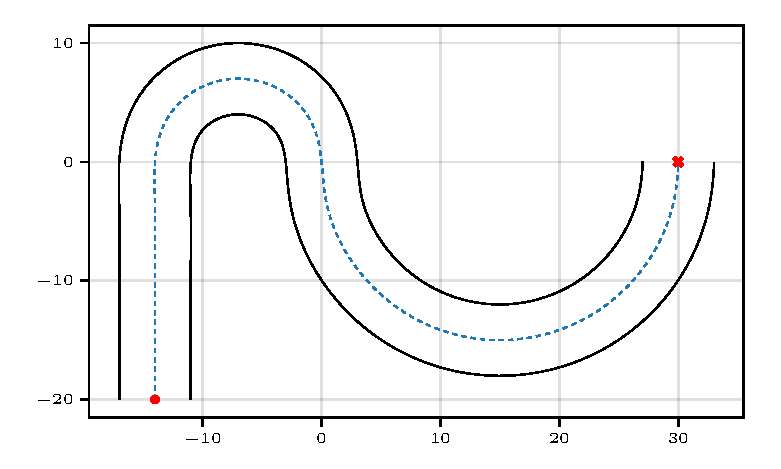
\includegraphics[width=1\textwidth]{../sync/massPointSteadyState/track.pdf}
    \caption{Test track used for the forward/backward pass example.}
    \label{fig:mass_point_track}
\end{figure}
\begin{figure}[H]
    \centering
    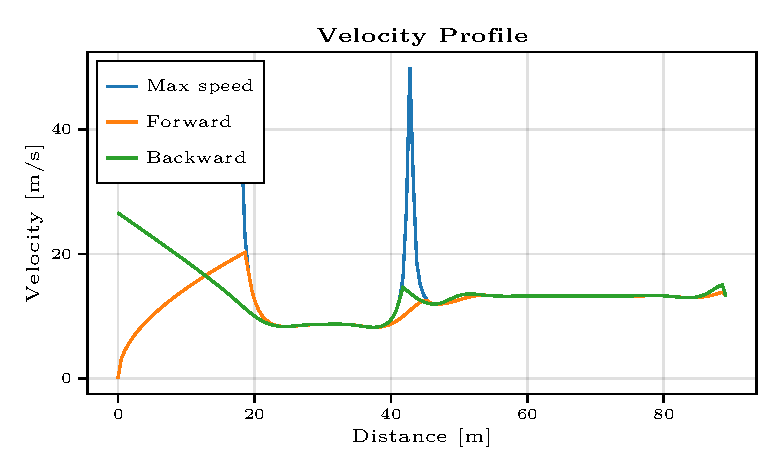
\includegraphics[width=1\textwidth]{../sync/massPointSteadyState/speed_profile.pdf}
    \caption{Speed profile from forward and backward passes with Quasi Steady state model}
    \label{fig:mass_point_speed_profile}
\end{figure}
Algorithm works in following manner:
\begin{enumerate}
    \item Maximum speed Pass: From the vehicle model and curvature along track, compute the maximum speed, blue line on Figure \ref{fig:mass_point_speed_profile}
    \item Forward pass: consider only forward acceleration limits of the vehicle (braking force is unlimited), run the vehicle from start to finish along the trajectory, applying maximum longitudinal acceleration and respecting max speed limit, orange line on Figure \ref{fig:mass_point_speed_profile}
    \item Consider only braking acceleration limits of the vehicle (acceleration force is unlimited), run the vehicle \emph{backwards, from finish to start} along the trajectory, applying maximum braking acceleration (braking now increases speed as the simulation is flipped)and respecting max speed limit
    \item Take minimum speeds of forward and backward pass and this gives the minimum time speed profile
\end{enumerate}
More complete description of this algorithm is in \cite{casanovaMinimumTimeVehicle2000}
This is the classic approach to minimum maneuvering time problem, the issue is that the trajectory of vehicle on track is fixed and cannot be optimized, the vehicle model must be heavily simplified, it does not work with any integral constraints like accumulator energy. However, the computation time can be fraction of a second for the entire lap. Tools using this method have proven to be extremely useful and many different analyses can be performed by leveraging its computational speed,for example varying the friction coefficient at on each corner, a corners importance on lap time can be calculated \cite{optimumg_corner_importance}. 
\section{Transcription methods}
Previous section described automotive specific methods of solving minimum maneuvering time problem, this section explains methods of transcribing the problem into the language of optimal control problem.
Transcription methods rewrite continuous (infinite-dimensional) OCP into finite-dimensional NLP.\@ That means representing the continuous trajectory of a state by values sampled at discrete points.
The terminology of transcription methods can be difficult to understand, as it is complex topic and often articles present conflicting information~\cite{kelly_traj_opt_terminology}. Website~\cite{kelly_traj_opt_terminology} and other work from Matthew Kelly~\cite{kelly_traj_opt_video,kelly_homepage,doi:10.1137/16M1062569} offers a very digestible introduction into the topic. This thesis focuses only on direct methods. Classification of methods in this thesis is based on~\cite{kelly_traj_opt_terminology} Figure~\ref{fig:ocp_methods_taxonomy} shows how transcription methods are commonly classified.

\begin{figure}[H]
\centering
\resizebox{\textwidth}{!}{%
\begin{tikzpicture}[
  >={Latex[length=2mm]},
  every node/.style={align=center},
  root/.style={draw, font=\footnotesize, text width=3.0cm, minimum height=0.8cm, inner sep=3pt},
  top/.style={draw, font=\footnotesize, text width=2.8cm, minimum height=1.0cm, inner sep=3pt},
  mid/.style={draw, font=\scriptsize, text width=2.6cm, minimum height=1.1cm, inner sep=3pt},
  leaf/.style={draw, font=\scriptsize, text width=2.0cm, minimum height=0.9cm, inner sep=2pt}
]
% --- Root ---
\node[root] (ocp) at (4.25, 0) {Continuous Time Optimal Control};

% --- Top-level branches: Direct on the left, Indirect center, HJB on the right ---
\node[top] (direct)   at (-1.0, -2.0) {Direct Methods:\\\textit{Transform into Nonlinear Program (NLP)}};
\node[top] (indirect) at ( 2.5, -2.0) {Indirect Methods, Pontryagin:\\\textit{Solve Boundary Value Problem}};
\node[top] (hjb)      at ( 6.0, -2.0) {Hamilton--Jacobi--Bellman Equation:\\\textit{Tabulation in State Space}};

\draw[->] (ocp.south) -- (direct.north);
\draw[->] (ocp.south) -- (indirect.north);
\draw[->] (ocp.south) -- (hjb.north);

% --- Direct children: shooting methods adjacent on the left, collocation on the right ---
\node[mid] (dss)  at (-4.0, -4.5) {Direct Single Shooting:\\\textit{Only discretized controls in NLP}\textit{}};
\node[mid] (dms)  at (-1.0, -4.5) {Direct Multiple Shooting:\\\textit{Controls and node start values in NLP}\textit{}};
\node[mid] (dcol) at ( 2.5, -4.5) {Direct Collocation:\\\textit{Discretized controls and states in NLP}\textit{}};

\draw[->] (direct.south) -- (dss.north);
\draw[->] (direct.south) -- (dms.north);
\draw[->] (direct.south) -- (dcol.north);

% --- Bottom leaves ---
\node[leaf] (erk1) at (-4.0, -6.7) {Explicit RK\\\textit{(integrator)}};
\node[leaf] (erk2) at (-1.0, -6.7) {Explicit RK\\\textit{(integrator)}};
\node[leaf] (hm)   at ( 1.4, -6.7) {$h$-methods\\\textit{low order,}\\\textit{many segments}};
\node[leaf] (pm)   at ( 3.6, -6.7) {$p$-methods\\\textit{high order,}\\\textit{few segments}};

\draw[->] (dss.south)  -- (erk1.north);
\draw[->] (dms.south)  -- (erk2.north);
\draw[->] (dcol.south) -- (hm.north);
\draw[->] (dcol.south) -- (pm.north);

\end{tikzpicture}%
}
\caption{Tree of approaches to continuous-time optimal control, adapted from~\cite{grosNumericalOptimalControla}, with the direct-methods branch expanded.}
\label{fig:ocp_methods_taxonomy}
\end{figure}

\subsection{Shooting methods}
Shooting methods get their name from aiming artillery canon analogy, with given powder load canon and target location find the aiming angle to hit the target. In depth explanation with animation and example code is here~\cite{kelly_cannon} This is classical boundary value problem. Methods shoot, miss, adjust aim, shoot again and iterate until target is hit. These methods are solving boundary value problem using an IVP solver. More precisely,
\begin{enumerate}
  \item Guess the controls
  \item Compute the solution using an initial value problem solver
  \item Compare the simulated value at the end of interval from 2.~with the boundary value(targets location)
  \item Based on error update the controls and go to 2.
\end{enumerate}

Shooting methods are split into single and multiple shooting. They differ in way they handle state discretisation. Single shooting discretizes the state only at start and end of interval and computes the trajectory in one shot. Whereas multiple shooting discretizes the states along the trajectory and computes multiple shots, this can be also parallelized on a CPU~\cite{FANG2022110926}. Shooting methods are progressively being displaced by collocation methods~\cite{raoSurveyNumericalMethods2010}

\subsection{Nonlinear Programming with Runge Kutta constraints}
These methods are not using initial value solvers to solve boundary value problem, instead they use nonlinear programming.
Most straightforward method to transcribe continuos optimal control problem
into non-linear program, is to use explicit Runge Kutta solving methods from
initial value problem as equality constraints on the dynamics of a vehicle. Using
Euler method, the constraints for the dynamics of vehicle are:
\begin{equation}
    \mathbf{x}_{k+1} = \mathbf{x}_k + h \cdot f(\mathbf{x}_k, \mathbf{u}_k),
\end{equation}
where $f$ denotes the vehicle dynamics, $h$ the step size, and $\mathbf{x}$ the state vector.
This works, but it may be the worst possible transcription method, due to high error and instability of euler method \cite{SolvingOrdinaryDifferential1987}. Problems of euler method encountered when solving initial value problems also translate to nonlinear programming. Implict RK methods can be used too, In Initial value problems they are used less often, as they require iterative solving. Optimal control problem is Boundary value problem and not initial value problem, therefore:

\begin{quote}
    \ldots for a boundary value problem \ldots any scheme becomes effectively implicit. Thus, the distinction between explicit and implicit initial value schemes becomes less important in the BVP context.
\end{quote}
\cite[p.~69]{Ascher1995}

For boundary value problem it makes no sense to use explicit Runge Kutta
methods, as they have inferior stability compared to implicit Runge Kutta
methods.\cite[p.~4]{raoSurveyNumericalMethods2010}. Implicit Runge Kutta methods, which are commonly used are from LobattoIIIA family, but any other method can be used. Book \cite{betts} uses
only these.

\subsection{Collocation methods}
\begin{quote}
    The concept of collocation is old and universal in numerical analysis \ldots For ordinary differential equations it consists in searching for a polynomial of de-gree s whose derivative coincides ("co-locates") at s given points with the vectorfield of the differential equation \ldots
    \cite[p.~224]{hairer}
\end{quote}
The article \cite{kelly_traj_opt_video} is an introductory explanation of inner working and implementation  of direct collocation methods, theory here is based on it and on \cite{garg_overview_nodate}. More in depth theory behind these methods was developed by Lloyd N. Trefethen in \cite{trefethenApproximationTheoryApproximation} and implementation in \cite{SpectralMethodsinMatlab}.
Collocation methods are a subset of implicit Runge-Kutta methods. The distinguishing property is that the solution of a boundary value problem is approximated by a piecewise polynomial in the independent variable (distance along the centerline). On each interval the polynomial is fixed by requiring it to satisfy the ODE exactly at $N$ chosen points the collocation nodes. 


There are numerous ways to construct a collocation method, in optimal control the classic methods are those based on roots Legendre or Chebyshev type I polynomials, Lagrange  polynomials \cite{ELGINDY199535, gargUnifiedFrameworkNumerical2010} and Gauss quadrature rule. In this thesis only Legendre and Gauss quadrature based collocation methods are covered. Figure \ref{fig:transcription_layer} depicts multiple ways of constructing collocation methods.

\begin{figure}[H]
\centering
\begin{tikzpicture}[
  >={Latex[length=2mm]},
  node distance=0.55cm and 0.18cm,
  basis/.style={draw, text width=1.4cm, minimum height=0.8cm, align=center, font=\scriptsize, inner sep=2pt},
  scheme/.style={draw, text width=3.2cm, minimum height=0.8cm, align=center, font=\small, inner sep=3pt},
  form/.style={draw, text width=1.25cm, minimum height=0.6cm, align=center, font=\scriptsize, inner sep=2pt},
  layer/.style={draw, minimum height=0.8cm, inner sep=4pt, align=center, font=\normalsize\bfseries}
]

\node[basis]                    (cheb) {Chebyshev\\I \& II};
\node[basis, right=of cheb]     (her)  {Hermite};
\node[basis, right=of her]      (lag)  {Laguerre};
\node[basis, right=of lag]      (leg)  {Legendre};
\node[basis, right=of leg]      (alag) {Assoc.\\Laguerre};
\node[basis, right=of alag]     (geg)  {Gegenbauer};
\node[basis, right=of geg]      (jac)  {Jacobi};

\node[layer, above=1cm of $(cheb.north)!0.5!(jac.north)$] (trans)
  {Orthogonal polynomials};

\foreach \n in {cheb,her,leg,lag,alag,geg,jac}
  \draw[->] (trans.south) -- (\n.north);

\node[scheme, below=1.8cm of leg] (lgr) {Legendre--Gauss--Radau\\(LGR) Quadrature};
\node[scheme, left=of lgr]   (lg)  {Legendre--Gauss\\(LG) Quadrature};
\node[scheme, right=of lgr]  (lgl) {Legendre--Gauss--Lobatto\\(LGL) Quadrature};

\draw[->] (leg.south) -- (lg.north);
\draw[->] (leg.south) -- (lgr.north);
\draw[->] (leg.south) -- (lgl.north);

\foreach \n in {cheb,her,lag,alag,geg,jac}
  \node[font=\Large, below=0.35cm of \n] {$\vdots$};

\foreach \parent in {lg,lgr,lgl}{
  \node[form, below=0.8cm of \parent, xshift=-0.85cm] (\parent-int)  {Integral};
  \node[form, below=0.8cm of \parent, xshift=0.85cm]  (\parent-diff) {Differ.};
  \draw[->] (\parent.south) -- (\parent-int.north);
  \draw[->] (\parent.south) -- (\parent-diff.north);
}

\end{tikzpicture}
\caption{Collocation transcription methods}
\label{fig:transcription_layer}
\end{figure}

\subsubsection{Lagrange polynomial}
First part of creating a collocation method is creating an interpolating polynomial basis,
\begin{equation}
    L_i(\tau) = \prod_{\substack{j=0 \\ j \neq i}}^{N} \frac{\tau - \tau_j}{\tau_i - \tau_j}, \qquad i = 0, \ldots, N.
    \label{legendre}
\end{equation}
Where $\tau$ is the point to be interpolated and $\tau_j$ and $\tau_i$ are node positions, in order to get interpolating polynomial $L(\tau)$, values at nodes $x_j$ are multiplied by corresponding Lagrange base and summed
\begin{equation}
    L(\tau) = \sum_{i=0}^{N} f_{i} L_i(\tau).
\end{equation}
Now it is possible to interpolate a state between the discretized nodes, Note that the node locations for Legendre polynomial are arbitrary. In the actual implementation, calculation of polynomial basis from definition \ref{legendre} is numerically impractical, therefore barycentric form from \cite{berrutBarycentricLagrangeInterpolation2004} has been used as implementation of these methods. The next step is to compute definite integral using values from function values at nodes.
%This creates a unique polynomial of lowest degree that interpolates a given set of data. The data points or nodes can be chosen arbitrary.
%A general RK method only yields state values at the stage points.
%Node choice is not arbitrary, nodes have to be selected in a special manner in order for second property of collocation to work. that is quadrature rule.
\subsubsection{Gaussian Quadrature rule}
Quadrature rule is the approximation of definite integral of a function by a sum of function values at given nodes. In optimal control context Gaussian quadrature is commonly used
\begin{equation}
    \int_{-1}^{1} f(\tau)\,\mathrm{d}\tau \approx \sum_{i=0}^{n} w_i \, f_i,
    \label{eq:gauss_quadrature}
\end{equation}
where $w$ are Gaussian quadrature weights.
A useful property of Gaussian quadrature of order $N$ is that it approximates the integral to machine precision whenever the integrated function is a polynomial of degree at most $2N-1$. Node selection for Gauss quadrature is \emph{not arbitrary}, in collocation methods the node positions are based on roots of Legendre polynomial. Node positions specify the type of collocation method and are creating in following manner.
%Pairing Gauss quadrature with Legendre polynomials creates a collocation method. Commonly used collocation methods constructed using Legendre polynomials and Gauss quadrature are constructed in following manner.
Let $P_N(\tau)$ denote the Legendre polynomial of degree $N$. Three node families are commonly used~\cite{garg_overview_nodate}:
\begin{itemize}
    \item Legendre-Gauss: roots of $P_N(\tau)$, includes no endpoints.
    \item Legendre-Gauss-Radau: roots of $P_{N-1}(\tau) + P_N(\tau)$, includes one endpoint.
    \item Legendre-Gauss-Lobatto: roots of $\dot{P}_{N-1}(\tau)$, includes both endpoints.
\end{itemize}

\begin{figure}
    \centering
    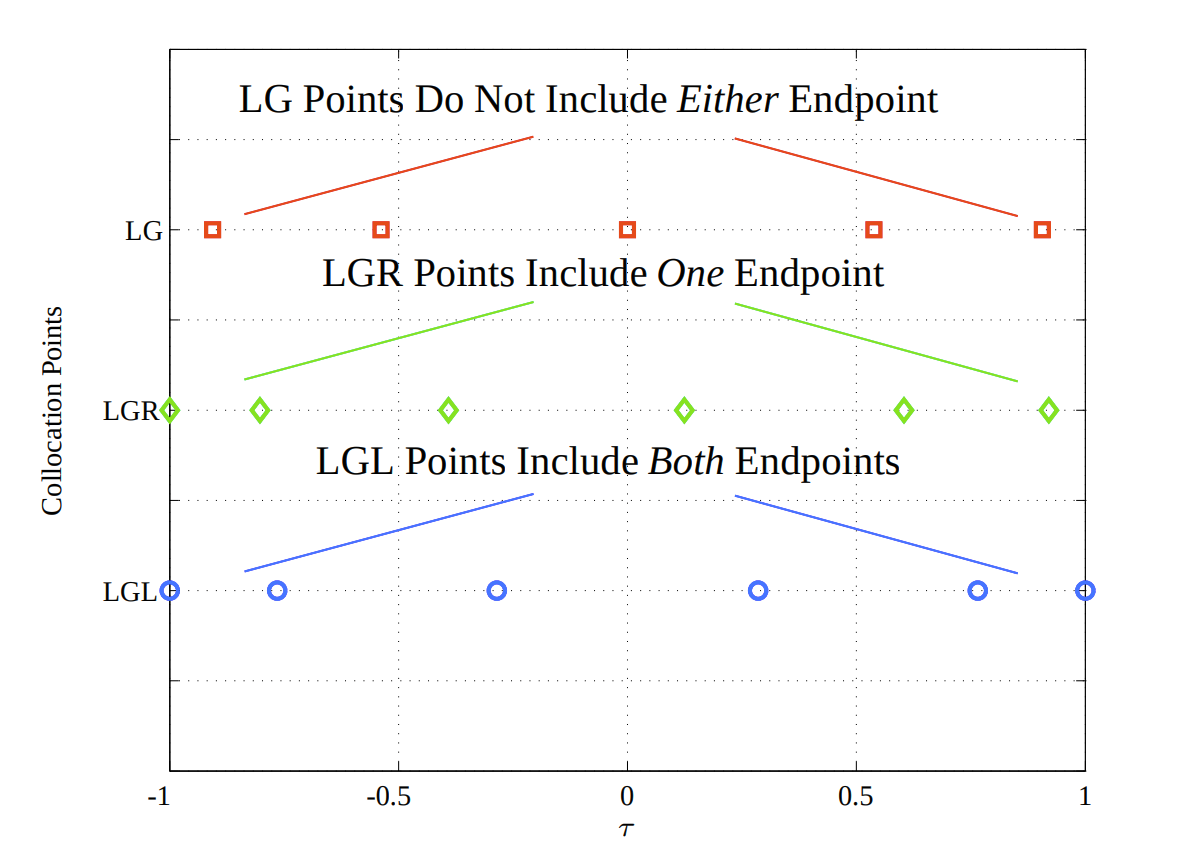
\includegraphics[width=0.75\linewidth]{../sync/image.png}
    \caption{Schematic Showing the Differences Between LGL, LGR, and LG Collocation Points, taken from \cite{garg_overview_nodate}}
    \label{fig:placeholder}
\end{figure}

\section{Collocation at Legendre-Gauss points}
%Legendre polynomials are paired with Gauss quadrature to create a collocation method.
%where $w_i$ are the quadrature weights and $f_i = f(\tau_i)$ are samples at the nodes. Because collocation and quadrature share nodes, quadrature of the collocation polynomial is exact up to the appropriate polynomial degree.
%https://en.wikipedia.org/wiki/Classical_orthogonal_polynomials#Table_of_classical_orthogonal_polynomials
%Collocation methods are the core of this thesis, I have implemented  Gauss radau, gauss, gauss lobatto. Collocation methods differ in points at which the derivative of polynomial coincides ("co-locates) with the vector field of differential equation. Commonly used methods in optimal control are radau, lobatto, legendre. They can be written in integral and differential form\cite{garg_overview_nodate}. Collocatiom methods in this thesis are based on Framework described in\cite{gargUnifiedFrameworkNumerical2010}

%Polynomial that aproximates the solution of ODE is based on Legendre polynomials.
Legendre-Gauss collocation methods uses nodes strictly inside the interval for approximation using polynomial.
With $N$ nodes, it is possible to approximate functions up to degree $N-1$ with machine precision.
States are approximated by series
\begin{equation}
    x^N_j(\tau) = \sum_{i=0}^{N} x_{ij}\, L_i(\tau),
\end{equation}
where $j$ is the number of the state.
Then the series is differentiated using barycentric form from~\cite[p.513]{berrutBarycentricLagrangeInterpolation2004} and evaluated at $k$-th collocation point $\tau_k$
\begin{equation}
    \dot{x}^N_j(\tau_k) = \sum_{i=0}^{N} x_{ij}\, \dot{L}_i(\tau_k) = \sum_{i=0}^{N} D_{ki}\, x_{ij}, \qquad D_{ki} = \dot{L}_i(\tau_k).
\end{equation}
Matrix $\mathbf{D} $is called \emph{Gauss Pseudospectral differentiation matrix}. In matrix notation can be written
\begin{equation}
\mathbf{DX} = \mathbf{F(X_{\mathrm{LG}}, U_{\mathrm{LG}})    }
\end{equation}
where $\mathbf{X_{LG}}$ is matrix of states at Legendre-Gauss node points, $\mathbf{U_{LG}}$ is matrix of controls at Legendre-Gauss node points, $\mathbf{X}$ is matrix of states at Legendre-Gauss node points and at initial point $x_0$

%then the output?? of differential equation can be aproximated using the
%differentiation matrix.
%\begin{equation}
%    \dot{x}^N_j(\tau_i) = (D\mathbf{X})_{ij}
%\end{equation}
This is then used as constraints to formulate a transcription method
\begin{equation}
    \begin{aligned}
        \min \quad        & \Phi(\mathbf{X}_{N+1})                         ,                                                \\
        \text{s.t.} \quad & \mathbf{DX} = \mathbf{F}(\mathbf{X}_\text{LG},\, \mathbf{U}_\text{LG})      ,                            \\
                          & \mathbf{X}_{N+1} = \mathbf{X}_0 + \mathbf{w^T} \mathbf{F}(\mathbf{X}_\text{LG},\, \mathbf{U}_\text{LG}), \\
                          & \mathbf{X}_0 = \mathbf{x}_0.
    \end{aligned}
\end{equation}
Where $w$ are the Gauss quadrate weights.
This is the differential form of Legendre-Gauss collocation method, integral from is described in \cite{gargUnifiedFrameworkNumerical2010}.
\section{Collocation at Legendre-Gauss-Radau points}
This method is constructed in similar manner to previous, with difference that one endpoint is a collocation node. This is an advantage, as the resulting nonlinear programming formulation does not require the gauss quadrature rule for endpoint and it is smaller.
This method approximates functions up degree $2N-2$ with machine precision, this is lower precision than Legendre-Gauss.
\begin{equation}
\begin{aligned}
\min \quad & \Phi(\mathbf{X}_N) \\
\text{subject to} \quad & \mathbf{D}\mathbf{X} = \mathbf{F}(\mathbf{X}^{\mathrm{LGR}}, \mathbf{U}^{\mathrm{LGR}}), \\
& \mathbf{X}_0 = \mathbf{x}_0.
\end{aligned}
\end{equation}
This is also a differential formulation.
\section{Collocation at Legendre-Gauss-Lobatto points}
The Gauss-Lobatto family includes both endpoints as collocation nodes and has a quadrature degree of exactness $2N-3$. It contains classical low-order schemes like the trapezoidal rule and Hermite--Simpson. I implement it using the Butcher tableau of LobattoIIIA implicit Runge--Kutta methods from \cite{ehlePadeApproximationsExponential}.

The dynamics is collocated at $N$ LobattoIIIA nodes $c_i \in [-1,1]$ with coefficient matrix $a_{ij}$ taken from the Butcher tableau. $\mathbf{X}_i$ and $\mathbf{U}_i$ are the state and control at node $i$, placed at $\tau_i = c_i h/2$, where $h$ is the length of the interval. The node constraints are
\begin{equation}
    \mathbf{X}_i = \mathbf{X}_0 + \frac{h}{2} \sum_{j=1}^{N} a_{ij}\, \mathbf{F}(\mathbf{X}_j, \mathbf{U}_j), \qquad i = 2, \dots, N,
\label{eq:lobattoIIIA-stage}
\end{equation}
where $\mathbf{X}_0$ is the left endpoint.
The resulting NLP is
\begin{equation}
\begin{aligned}
\min \quad & \Phi(\mathbf{X}_N) \\
\text{subject to} \quad & \mathbf{X}_i = \mathbf{X}_0 +  \sum_{j=1}^{N} a_{ij}\, \mathbf{F}(\mathbf{X}_j, \mathbf{U}_j), \quad i = 2, \dots, N, \\
& \mathbf{X}_0 = \mathbf{x}_0.
\end{aligned}
\end{equation}
This is an integral formulation of collocation method, in book \cite{betts} trapezoidal and Hermite-Simpson methods written in this form.

%\section{Gauss methods as pseudospectral collocation}
%I have implemented Gauss-Legendre, Gauss-Lobatto, Gauss-Radau as global collocation methods, that is one polynomial approximating the entire trajectory. I have implemented them according to~\cite{garg_overview_nodate}
%\section{Gauss methods as h-method}
%\subsection{collocation integral form}
%integral form is straight forward, same as other unge kutta Methods
%\subsection{collocation differential form}
%differeanital form requires to create differentiation matrix of the
%aproximating polnomial,which contains the difference of the approximating
%polynomial.

\subsection{h and p methods for collocation}
A function can be approximated in three ways. The first uses a single high-order polynomial over the entire trajectory, these are p methods. The second uses many piecewise continuous polynomials of low and fixed order, as in \cite{betts}, these are h methods. The third combines both ideas, using many polynomials whose order is allowed to vary between segments, these are hp methods. The Legendre-Gauss, Legendre-Gauss-Radau and Legendre-Gauss-Lobatto schemes presented above are the building blocks for all three categories. A single global instance gives a p method. Chaining many low-order instances on consecutive intervals with continuity at the shared endpoints gives an h method. Chaining instances of different orders gives an hp method.

Intuitively p methods should suffer from the Runge phenomenon, but they do not. The discretization nodes are not equispaced, they are clustered toward the endpoints, which suppresses the oscillations. Methods based on roots of Chebyshev polynomials suppress the Runge phenomenon better than Legendre methods\cite{trefethenApproximationTheoryApproximation}.
\section{Mesh refinement methods}
Mesh refinement works by changing polynomial order and number and place of segements. In mesh refinemnt it is also important to remove segments that are unecessary. Mesh refinemnt methods are divided into three categories.
\begin{figure}[H]
\centering
\begin{tikzpicture}[
  >={Latex[length=2mm]},
  node distance=0.7cm and 0.35cm,
  method/.style={draw, text width=2.4cm, minimum height=0.9cm, align=center, font=\small, inner sep=3pt},
  layer/.style={draw, minimum height=0.8cm, inner sep=4pt, align=center, font=\normalsize\bfseries}
]

\node[method]              (p)   {$p$-refinement\\(raise polynomial degree)};
\node[method, right=of p]  (h)   {$h$-refinement\\(subdivide segments)};
\node[method, right=of h]  (hp)  {$hp$-refinement\\(combination of h and p)};

\node[layer, above=1cm of $(p.north)!0.5!(hp.north)$] (mesh)
  {Mesh refinement strategy};

\foreach \n in {p,h,hp}
  \draw[->] (mesh.south) -- (\n.north);

\end{tikzpicture}
\caption{Mesh refinement categories~\cite{darbyHpAdaptivePseudospectral2011,pattersonPhMeshRefinement2015}.}
\label{fig:mesh_refinement_layer}
\end{figure}



\subsection{P adaptive methods}
The p adaptive methods work by increasing the order of polynomial, until the error
is below user defined threshold. Figure \ref{fig:power_node_controls} shows that
error along track is not distributed equaly. Error is localised around areas
with large jump in controls. These areas need finer sampling. P methods cannot
focus these specific points directly, they focus entire trajectory.

The errors are concentrated around the discontinuity of controls, where the
behaviour of the vehicle is more complex/ requiring high order or finer
approximation see Figure \ref{fig:power_node_controls}. Time optimal control of car around track has many discontinuities and therefore p methods are not a good fit for this use.

\begin{figure}[H]
    \centering
    \makebox[\textwidth][c]{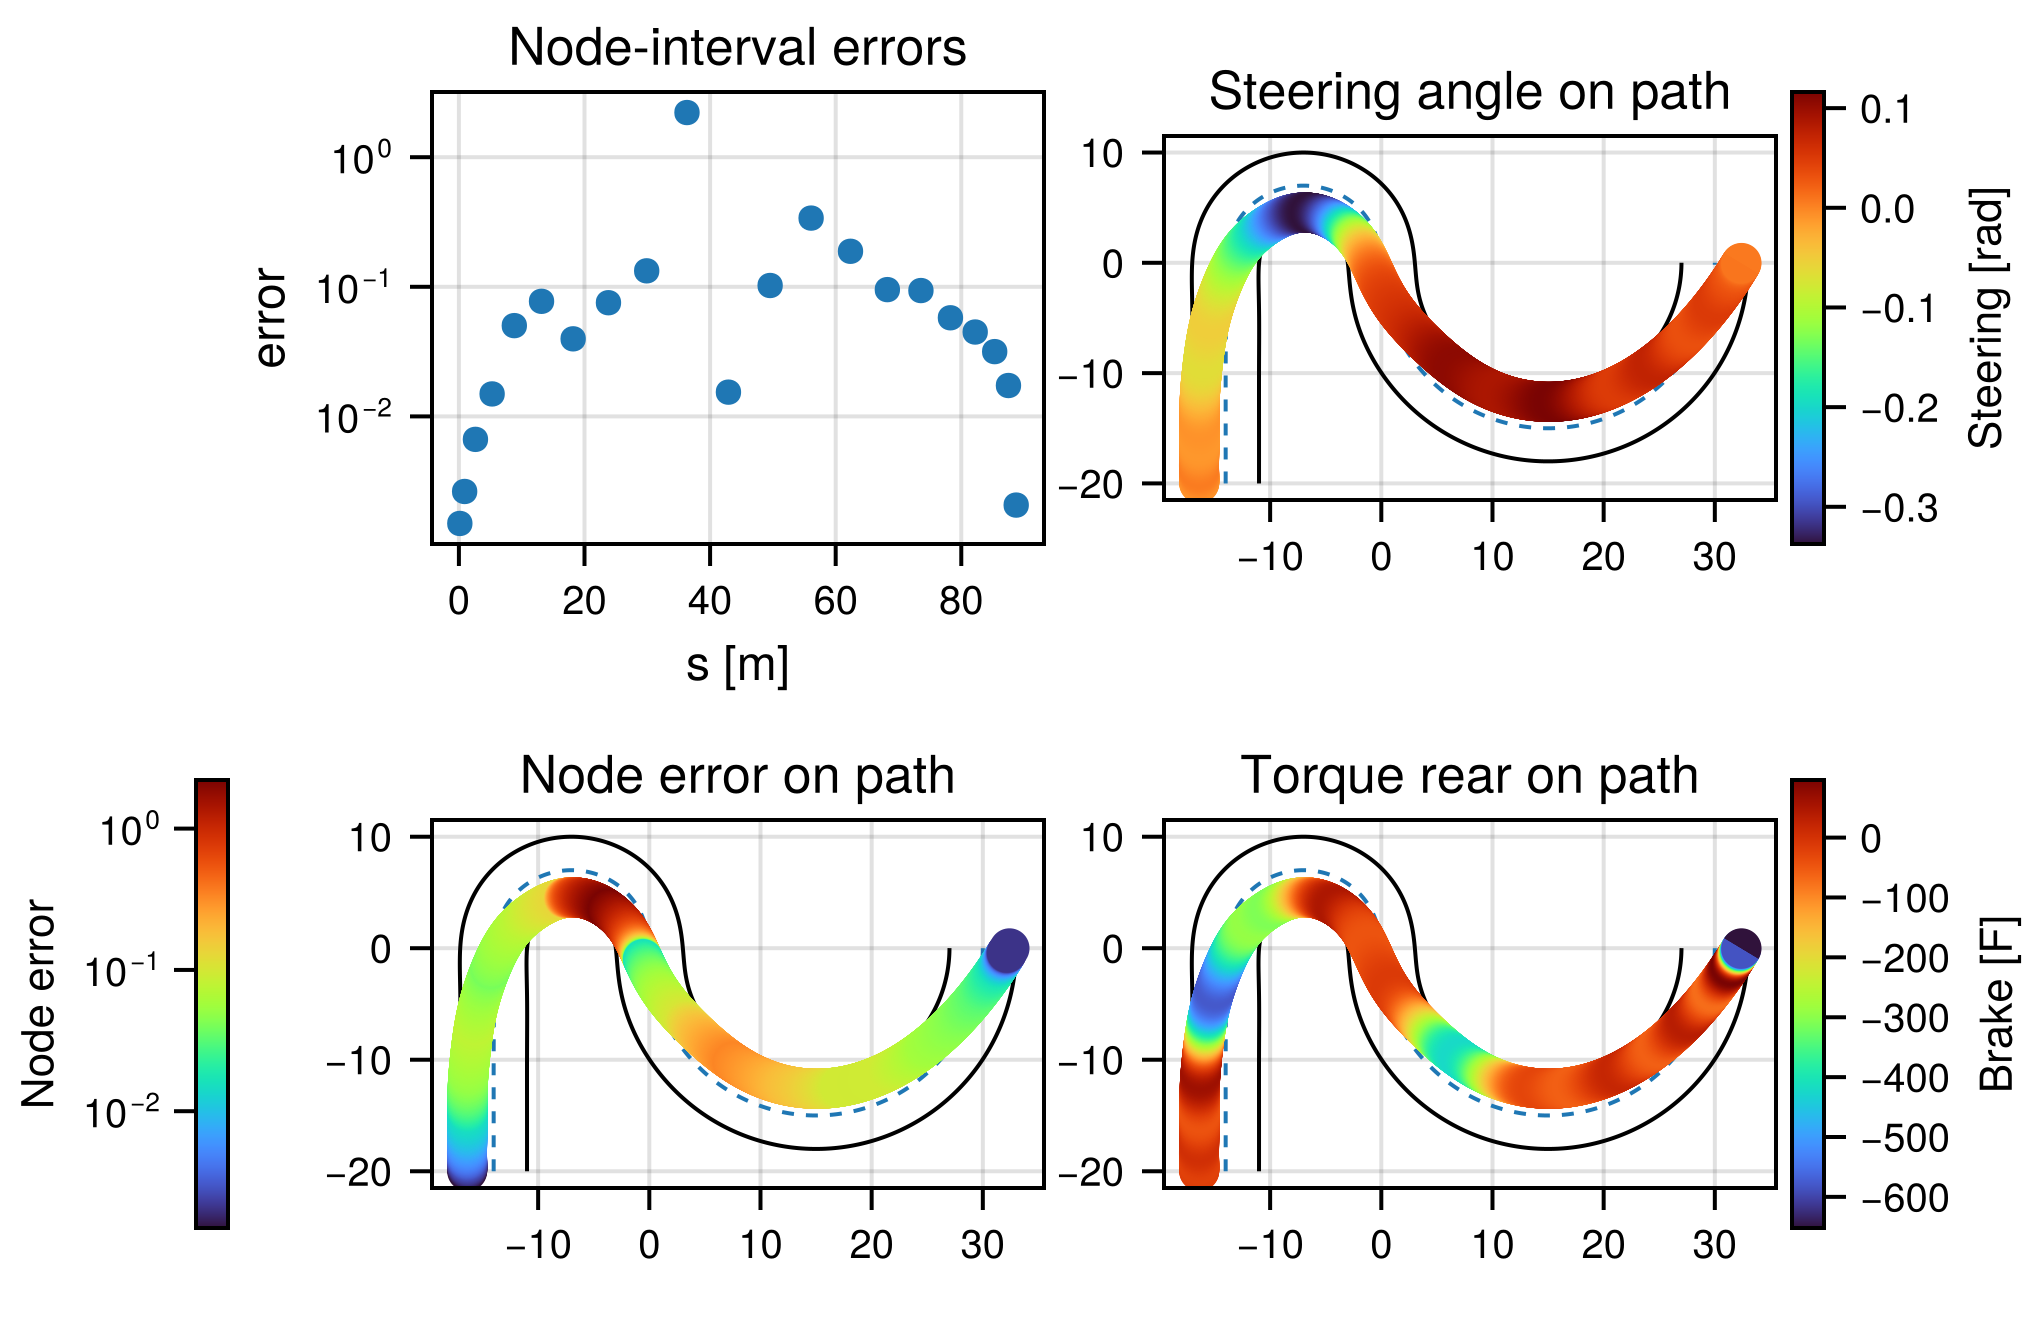
\includegraphics[width=1\textwidth]{../sync/p_methodplots/power_summary2x2.png}}
    \caption{Node-interval ODE error for power-test case.}
    \label{fig:power_node_controls}
\end{figure}

\subsection{h adaptive methods}
The h methods are used when solution of optimal control problem is approximated by
many intervals with low degree polynomial. These methods can decide to split
segment into two smaller segments, they use different techniques to do this.
Method described in \cite{betts} calculates error using Romberg quadrature with machine precision. Another
method described in \cite{jisongzhaoshuangliAdaptiveMeshRefinement} uses
techniques from essentially non oscillatory (ENO) interpolation

\begin{figure}[H]
    \centering
    \makebox[\textwidth][c]{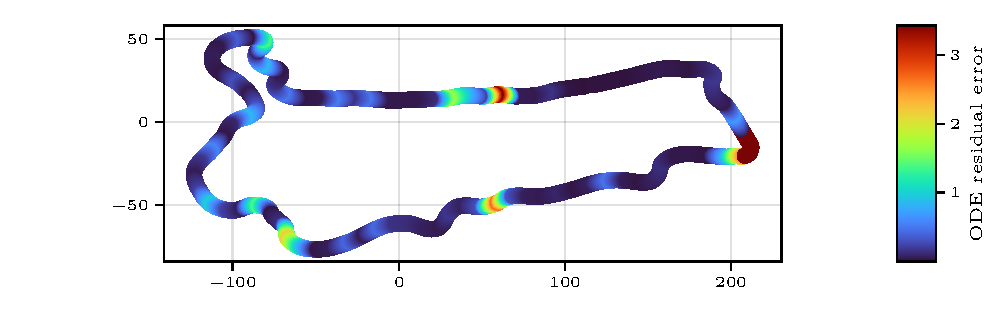
\includegraphics[width=1\textwidth]{../sync/thesisImages/mesh_refinement_fscz_error_iter0.pdf}}
    \caption{Node-interval ODE error for power-test case.}
    \label{fig:power_node_controls}
\end{figure}

\begin{figure}[H]
    \centering
    \makebox[\textwidth][c]{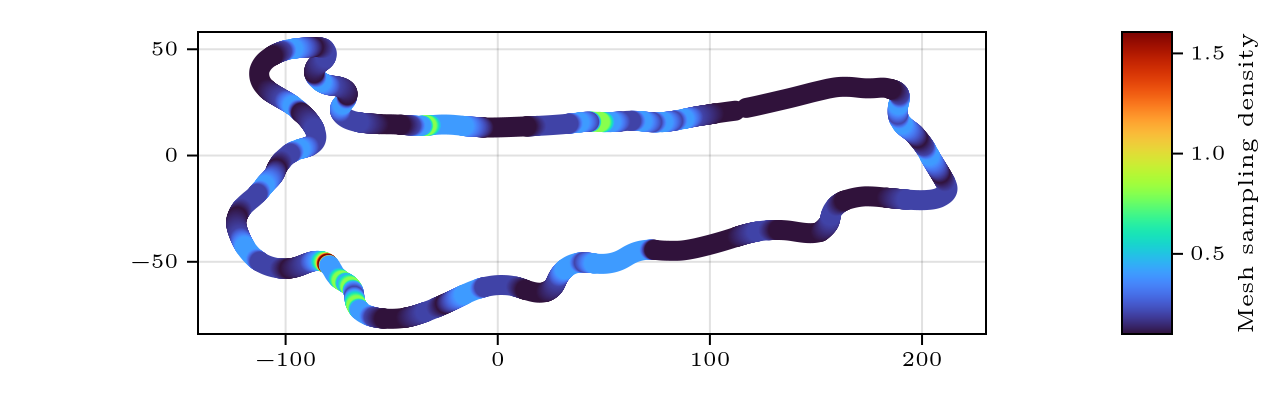
\includegraphics[width=1\textwidth]{../sync/thesisImages/mesh_refinement_fscz_density_iter10.png}}
    \caption{Node-interval ODE error for power-test case.}
    \label{fig:power_node_controls}
\end{figure}

\cite{Harten1997} to decide where to split and remove nodes.
\subsection{hp adaptive methods}
The hp adaptive methods are state of the art in mesh refinement. They are
combination of increasing/decreasing mesh segments and increasing/decreasing
order of approximating polynomial inside segments. One of the first hp-method
and commonly cited is decribed in
article~\cite{darbyHpAdaptivePseudospectral2011} from University of Florida.
They have produces numerous papers on hp- adaptive mesh
refinemnt~\cite{agamawiCGPOPSSoftwareSolving2020}
\cite{liuAdaptiveMeshRefinement2018}. Recent work on mesh refinemnt for
functions with kinks~\cite{wilkaAdaptiveHpPolynomialBased2025}. They are the
most complex for implementation and unfortunately I did not have the time to
implement them.

\section{Adjoint methods}
\label{sec:adjoint}

Adjoint methods allow for differentiating the solution of optimization problem.
In this case it is function of time on states and controls along the trajectory and car parameters This is very useful as it greatly simplifies sensitivity
analysis. Traditional way of sensitivity analysis is to compute several runs with
different vehicle parameters, but this allows to compute sensitivity of all
parameters in one shot. I am using DiffOpt.jl \cite{besancon2023diffopt}, it is
not exactly adjoint i dont really understand very well how it works.

\chapter{Solvers for nonlinear programming}
Once the objective function and constraints are created, the problem is passed
to the NLP solver. Popular methods are Lagrange-Newton methods, these are sequential quadratic solvers and
interior point solvers. These solvers are perhaps the most complex component used in this thesis, this chapter will cover them at high leve, as full theory is beyond the scope. A comprehensive overview of Lagrange-Newton methods is in article\cite{vanaret_implementing_2025}, where the methods are broken down into key algorithmic components and unifying framework of solvers is presented. Figure\ref{fig:wheel} shows the key algorithmic components.
\begin{figure}[H]
    \centering
    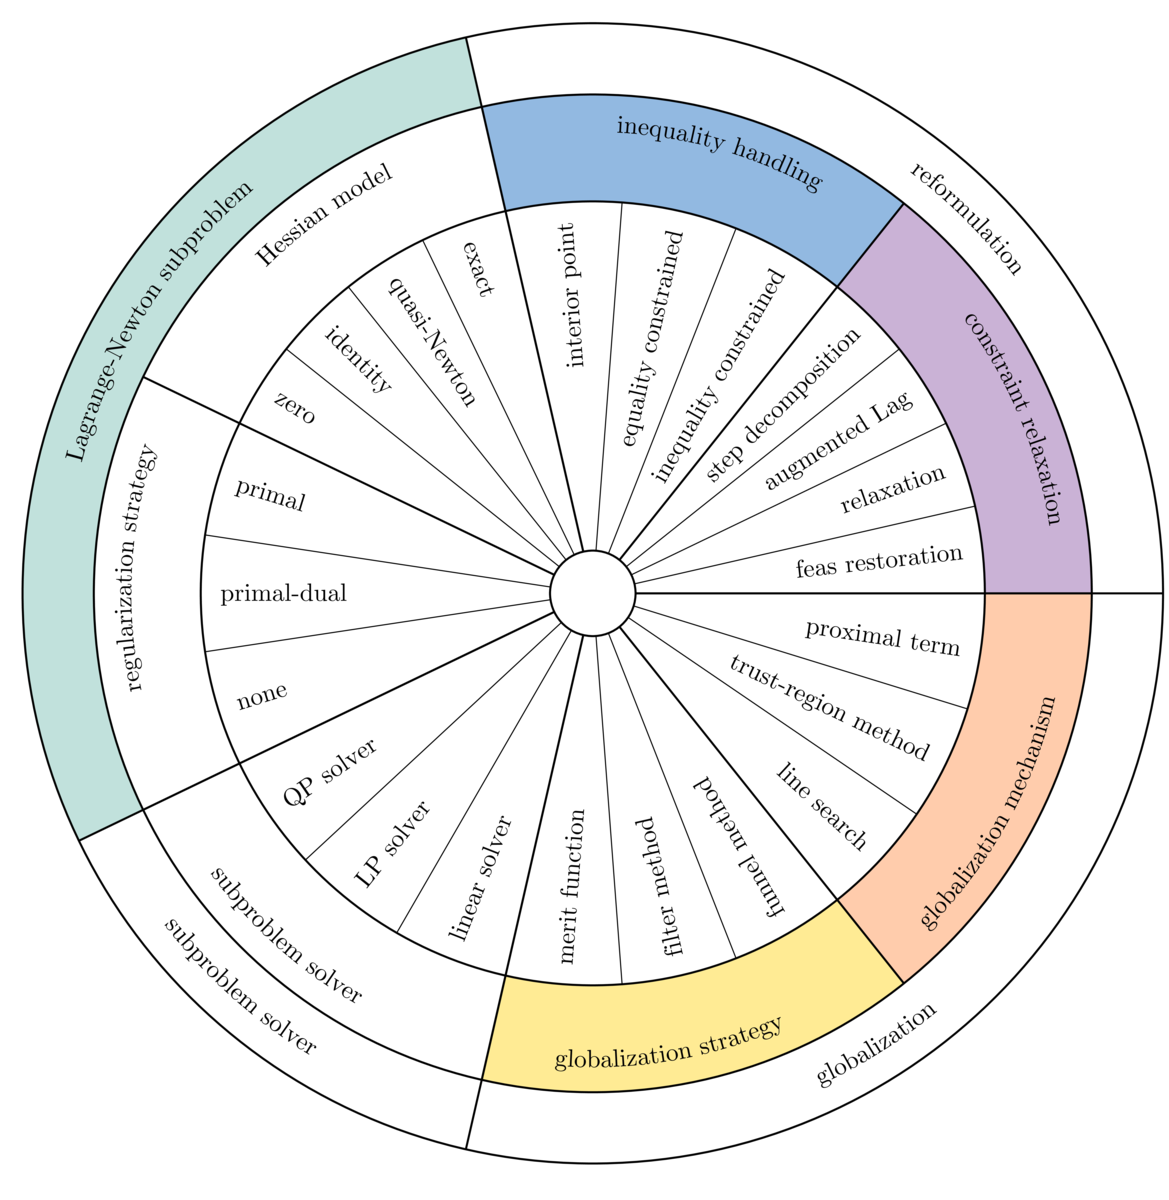
\includegraphics[width=0.8\textwidth]{figures/wheel.png}
    \caption{Unifying framework: the “wheel of strategies”\cite{vanaret_implementing_2025}}
    \label{fig:wheel}
\end{figure}
High level overview required for this thesis of Lagrange-Newton methods is in Figure \ref{fig:nlp_flowchart}. 

\begin{figure}[H]
\centering
\resizebox{\textwidth}{!}{%
\begin{tikzpicture}[
  >={Latex[length=2mm]},
  node distance=0.8cm and 0.3cm,
  every node/.style={font=\small, align=center},
  box/.style={draw, minimum height=0.8cm, inner sep=4pt},
  problem/.style={box},
  branch/.style={box, font=\small\bfseries},
  stagebox/.style={box},
  deriv/.style={box, font=\small, text width=2.2cm},
  terminal/.style={box, line width=1pt}
]

\node[problem] (nlp) {NLP problem statement};

\node[branch, below left=1.2cm and 2.2cm of nlp] (sqp) {Sequential Quadratic programming};
\node[branch, below right=1.2cm and 2.2cm of nlp] (ipm) {Interior point methods};

\node[stagebox, below=of sqp] (qp) {Quadratic model of Lagrangian,\\linearized constraints,\\QP subproblem};
\node[stagebox, below=of ipm] (bar) {Barrier problem reformulation};

\node[problem, below=3.5cm of nlp] (need) {Calucate first and second derivatives};

\node[deriv, below=1.6cm of need] (fd) {Finite\\differences};
\node[deriv, left=of fd]  (sym)  {Symbolic\\(CAS)};
\node[deriv, left=of sym] (anal) {Analytic\\(hand-coded)};
\node[deriv, right=of fd] (ad)   {Automatic differentiation};
\node[deriv, right=of ad] (qn)   {Quasi-Newton Approximation};

\node[terminal, below=4cm of need] (newton) {Assemble linear system of equations\\\textbf{Newton step}};

\draw[->] (nlp) -- (sqp);
\draw[->] (nlp) -- (ipm);
\draw[->] (sqp) -- (qp);
\draw[->] (ipm) -- (bar);
\draw[->] (qp)  -- (need);
\draw[->] (bar) -- (need);

\draw[->] (need) -- (anal);
\draw[->] (need) -- (sym);
\draw[->] (need) -- (fd);
\draw[->] (need) -- (ad);
\draw[->] (need) -- (qn);

\draw[->] (anal) -- (newton);
\draw[->] (sym)  -- (newton);
\draw[->] (fd)   -- (newton);
\draw[->] (ad)   -- (newton);
\draw[->] (qn)   -- (newton);

\end{tikzpicture}}
\caption{NLP solution flow: problem statement $\to$ solver family (SQP / IPM) $\to$ derivative computation $\to$ assembled Newton step.}
\label{fig:nlp_flowchart}
\end{figure}



\section{Nonlinear programming}

General NLP problems can be written as:
\begin{equation}
    \begin{aligned}
        \min_{\mathbf{x} \in \mathbb{R}^n} \quad & f(\mathbf{x})                 \\
        \text{s.t.} \quad                        & \mathbf{h}(\mathbf{x}) = 0    \\
                                                 & \mathbf{g}(\mathbf{x}) \leq 0
    \end{aligned}
    \label{eq:general_nlp}
\end{equation}

Here $\mathbf{x} \in \mathbb{R}^n$ is the decision-variable vector, $f : \mathbb{R}^n \to \mathbb{R}$ is the scalar objective, $\mathbf{h} : \mathbb{R}^n \to \mathbb{R}^m$ stacks the $m$ equality constraints, and $\mathbf{g} : \mathbb{R}^n \to \mathbb{R}^p$ stacks the $p$ inequality constraints. In the lap-time setting $\mathbf{x}$ holds the discretised states and controls, $f$ is total lap time, $\mathbf{h}$ enforces vehicle dynamics and boundary conditions, and $\mathbf{g}$ enforces track limits, tire friction circle and actuator bounds.

\subsection{KKT conditions}
KKT condiitons are the conditions of optimality, if satisfied the point is local optimum.
alpha and omega of nolinear programming, lord praise the KKT conditions.

\begin{equation}
    \begin{aligned}
        \nabla f(\mathbf{x}) + \sum_{i=1}^{m} \lambda_i \nabla h_i(\mathbf{x}) + \sum_{i=1}^{p} \mu_i \nabla g_i(\mathbf{x}) & = 0                            \\
        \mathbf{h}(\mathbf{x})                                                                                               & = \mathbf{0}                   \\
        \mathbf{g}(\mathbf{x})                                                                                               & \leq \mathbf{0}                \\
        \mu_i                                                                                                                & \geq 0, \quad i = 1, \ldots, p \\
        \mu_i g_i(\mathbf{x})                                                                                                & = 0, \quad i = 1, \ldots, p
    \end{aligned}
\end{equation}


%\begin{equation}
%    \begin{pmatrix}
%        \nabla^2 \mathcal{L} & A^T \\
%        A                    & 0
%    \end{pmatrix}
%    \begin{pmatrix}
%        -\Delta x \\
%        \lambda
%    \end{pmatrix}
%    =
%    \begin{pmatrix}
%        \nabla f(x) \\
%        c(x)
%    \end{pmatrix}
%\end{equation}

\section{Interior point methods: IPOPT, MadNLP}
\label{sec:interior_point}

Interior point solvers or barrier solvers work by reformulating the NLP into a
barrier problem at each step and solving a sequence of these barrier problems, with decreasing
barrier parameter. Solver used in this thesis is IPOPT \cite{wachter_implementation_2006} and MadNLP\cite{shin2024accelerating}.

\subsection{Barrier problem formulation}
\label{subsec:barrier_problem_formulation}
There are multiple ways to transform NLP in to barrier problem, this section
will briefly describe how IPOPT does it.
IPOPT article~\cite{wachter_implementation_2006} Describes how to transform generic
NLP into form~\ref{eq:barrier_problem} 

\begin{equation}
    \begin{aligned}
        \min_{\mathbf{x} \in \mathbb{R}^n} \quad & \phi_\mu(\mathbf{x}) := f(\mathbf{x}) - \mu \sum_{i=1}^{n} \ln(x_i^{(i)}) \\
        \text{s.t.} \quad                        & c(\mathbf{x}) = 0
    \end{aligned}
    \label{eq:barrier_problem}
\end{equation}

 The Lagrangian of the barrier problem is defined as
\begin{equation}
    \mathcal{L}(\mathbf{x}, \lambda, z) := f(\mathbf{x}) + c(\mathbf{x})^\top \lambda - z.
    \label{eq:lagrangian_barrier}
\end{equation}
Then barrier problem is further transformed into set of linear equations, a KKT linear system, that
computes the Newton step:
\begin{equation}
    \begin{bmatrix}
        W_k   & A_k & -I  \\
        A_k^T & 0   & 0   \\
        Z_k   & 0   & X_k
    \end{bmatrix}
    \begin{bmatrix}
        d_x^k       \\
        d_\lambda^k \\
        d_z^k
    \end{bmatrix}
    = -
    \begin{bmatrix}
        \nabla f(x_k) + A_k \lambda_k - z_k \\
        c(x_k)                              \\
        X_k Z_k e - \mu_j e
    \end{bmatrix}.
\end{equation}
Here $W_k = \nabla^2 \mathcal{L}(x_k, \lambda_k, z_k)$ is the Hessian of the Lagrangian, $A_k$ is the Jacobian of the equality constraints $c(x)$ and $\nabla f(x_k)$ is the gradient of the objective. The unknowns $d_x^k$, $d_\lambda^k$ and $d_z^k$ are the Newton steps in the primal variables, equality multipliers and bound multipliers; $\mu_j$ is the barrier parameter, which is driven to zero across outer iterations.

There are numerous commercial and free algorithms to solve this. For smaller
systems it is LU decomposition, but for larger sparse problems a dedicated
solver is a must. IPOPT is most commonly used with MUMPS \cite{MUMPS:1} solver
which is free. There are several linear commercial solvers, Harwell Subroutine
Library(HSL) offers ma27 ma87 ma97 \cite{hsl2011collection}.Panua technologies offers PARDISO solver
\cite{pardiso}. Harwell Subroutine Library solvers are available free for
academic usage and PARDISO solver is available free for academic usage. Latter solvers run on CPU, Nvidia has linear solver CuDSS\cite{nvidia_cudss} which runs on GPU.
Linear solver are capable of multithreading on CPU, which needs to be explicitly
turned on. 

\section{Sequential quadratic programming}
Sequential quadratic programming is less commonly used for offline trajectory optimisation, usage of IPOPT prevails.

\section{Calculation of derivatives}
Major complication of many Lagrange-Newton methods is that they require gradient of the objective function, Jacobian of the constraints and Hessian of the Lagrangian to compute the Newton step. Computing these derivatives can be time intensive. The most universal method is finite differences, which means evaluating the function around the current point and estimating the derivative, this works even for a black box model, but the derivatives are not exact. When the model is available, symbolic differentiation can be used, however, the full symbolic expression is often too large to be evaluated effectively due to repeated chain and product rules. Automatic differentiation aims to solve the problems of previous methods, by applying the chain rule to the elementary operations of a function. A comprehensive review of automatic differentiation is given in~\cite{cortildBriefReviewAutomatic2023}.


\section{Scaling and matrix conditioning}
Common pitfall of nonlinear programming is poor scaling. This happens when the
solver encounters variables, that are orders of magnitude apart, for example
motor force in thousands of newton and heading angle in radians. This happens,
because at the core of nonlinear programming solver is a linear solver WROOOOONG elipsa zoptimalziace to inka ukazuje
(MUMPS,MA97,PARDISO,...), that has to do matrix factorization every iteration,
to solve KKT linear system. If this linear system is ill conditioned due to
improper scaling, the factorization may be imprecise and search direction
corrupted.

Another thing which led to issues is constraints qualification. Linear
indpendence constiant qualification requires gradients of the active
constraints to be linearly independent. If it is violated, the jacobian of the constraints is
rank deficient and linear solve may fails

\section{sparsity}
Sparsity is good, sparsity means matrix hessians and jacobians with many zeros
also sparsisty in constraints, that means not having super very long expression
with many terms in constraint. I guess it is beacause deriavtive is difficult
then and can lead solver in wrong direction or take small stages. Therefore
using more decison variables to define same problem can actually lead to faster
computation \cite{julia_discourse_ipopt_hessian}. Certain solvers can exploit
the sprasity strcuture, such as FATROP\cite{vanroyeFATROPFastConstrained2023}.
In source \cite{jorisgillisIPOPTSteroidsFatrop2024} Joris gillis a casadi
developer compares IPOPT to FATROP, with \textbf{FATROP being 33 times faster
    on a trajecotry optimisation problem.}

Also \cite{betts} describes how sprasity structure helps with afster hessian
aprprixmiation for using finite difference??? secant method.

\section{Initialization}
NLP solvers require initial guess for all decision variables, to start solving.
For this problem initial guess is obtained driving the vehicle on given track.
PD controller is used to keep the car on the centerline and P controller is
used to keep velocity at 5m/s. In general, it is possible to initialize all
variables at zero, but with large scale nonlinear programming this approach is
not used. For this problem initialization with zeros leads to singularity in
equation \ref{time2path} and is not possible at all. must be ineitialzied
otherwise very baaaadt?

\section{Global and local optimums}
This optimization problem is generally non convex, therefore any local optimum
does not guarantee global optimum.Commonly used NLP solvers, like IPOPT
guarantee only local optimums and not global ones. Good initization is basis
for finding a local optimum close to the global optimum. Source?????

\part{Implementation of Optimal Control problem}
\chapter{Frameworks for Optimal Control Problem Formulation}
Process of solving optimal control problem has 3 parts. Problem defintion,
solving of nonlinear program, optional mesh refinment

\begin{figure}[h]
  \centering
  \begin{tikzpicture}[
      node distance=1.4cm,
      block/.style={rectangle, draw, thick, font=\small, minimum width=4cm, minimum height=0.9cm, align=center, fill=white},
      exit/.style={ellipse, draw, thick, font=\small, minimum width=3cm, minimum height=0.8cm, align=center, fill=white}
    ]
    \node[block] (def) {1. Problem definition};
    \node[block, below=of def] (nlp) {2. NLP solve};
    \node[block, below=of nlp] (mesh) {3. Mesh refinement (optional)};
    \node[exit, below=of mesh] (sol) {Solution};
    \draw[->, thick] (def) -- (nlp);
    \draw[->, thick] (nlp) -- (mesh);
    \draw[->, thick] (mesh) -- node[right, font=\small]{converged} (sol);
    \draw[->, thick] let \p1=(mesh.east), \p2=(nlp.east) in
    (mesh.east) -- (\x1+1.5cm,\y1) -- node[right, font=\small, align=left]{needs\\ refinement} (\x1+1.5cm,\y2) -- (nlp.east);
  \end{tikzpicture}
  \caption{Optimal control problem solving pipeline.}
  \label{fig:ocp-pipeline}
\end{figure}

The concensus in optimal control community about tools for prolbem formulation
is that:
\begin{quote}
  There is no shortage of optimal control software based on pseudospectral approaches. There are a number of other optimal control libraries that tackle similar kinds of problems, such as OTIS4, GPOPS-II,and CASADI.
\end{quote}
\cite{Falck2021}\cite{DymosDocs}
This chapter is aobut tool that define the OCP, and supply derivatives of the problem, they cannot solve the problem by themselves.
\section{GPOPS-II}
GPOPS-II \cite{pattersonGPOPSIIMATLABSoftware2014} is perhaps the most advaced
tool for otimal control, it was developed ad University of Florida by Michael
patterson and Anil V. Rao. other tools allows defininng the problem, but
GPOPS-II is a level higher. It also includes advanced mesh refinement
strategies, multiple phase OCP and automatic scaling. For solving the problem
it uses IPOPT or SNOPT. It interaces with MATLAB and C++, uses ADigator
\cite{weinstein2017algorithm} for automatic differetnation. This tool is
commercial and closed source. Implementaion in this thesis is heavily based on
work of community from University of Florida.
\section{CasADi}
CasADi is an open-source tool for nonlinear optimization and algorithmic
differentiation.\cite{CasADi}\cite{anderssonCasADiSoftwareFramework2019}.
interfaces with C++,Python,MATLAB. It provides a framework INE SLOVO to build
the problem, and calculate the hessian and jacobian for nlp solver it does not
have any mesh refinemnt algorithms. Commonly paired with IPOPT for nonliner
programming, but is compatible with large variety of solvers.

\section{dymos + OpenMDAO}
Python has hp mesh refinemnt uses OpenMDAO \cite{Gray2019a} developed at NASA
Glenn research center for evaluating aircraft concepts. Lobatto and radau
collocation as default \cite{Falck2021}. According to forum post from julia
discourse, which may be biased towards julia it is slower compared to infiteOpt
in julia \cite{DoesAnybodyKnow2024}. But it has mesh refinemnt so that is good.
\section{Acados}

\cite{Verschueren2021}

\section{Julia + JuMP/ infititeopt/ examomdels}
ExaModels, JuMP

JuMP is the go to tool for algebraic modelling in julia, it is mature,
versatile. Supports Linear programming, quadartic programming, mixed linear
programming, Nonlinear programming. ExaModels \cite{shin2023accelerating} is a
specialized algebraic modelling tool, it utilisies Single instruction, multiple
data methods,enabling derivative evaluation on GPU accelerators. Coupled with
MadNLP solver, the entire computation of nonlinear optimisation can be run on a
GPU.

Julia options
\begin{enumerate}
  \item Julia + jump
  \item Julia + jump + infinte opt
  \item julia + ExaModels
\end{enumerate}

Infite opt already has various collocation methods implemented. For learning
purposes and in fear that in future down the road i would realise that
infniteopt blocks all the stuff i want to do i decided to use jump, without
infite opt.

No julia package has  mesh refinement
I chose julia + jump,


\begin{table}[h]
  \centering
  \small
  \begin{tabular}{|p{4.5cm}|p{4.5cm}|p{4.5cm}|}
    \hline
    \textbf{Aspect} & \textbf{Julia + JuMP + InfiniteOpt} & \textbf{Python + OpenMDAO + dymos} \\
    \hline
    Language / runtime
      & Julia, JIT-compiled, no GIL
      & Python, interpreted, GIL (NumPy releases) \\
    \hline
    License
      & MIT (all components)
      & Apache 2.0 \\
    \hline
    Algebraic modelling style
      & Macro-based (\texttt{@variable}, \texttt{@constraint}, \texttt{@objective})
      & Component graph (\texttt{ExplicitComponent}, \texttt{Group}, promotes/connects) \\
    \hline
    Derivatives
      & AD via MathOptInterface; sparsity from expression graph
      & MAUD unified derivatives; mix analytic / AD / FD / complex-step per component, framework chains them \\
    \hline
    Transcription methods
      & Finite difference (Forward, Central, Backward); orthogonal collocation on finite elements with Gauss--Lobatto nodes only
      & Radau pseudospectral, Gauss--Lobatto, explicit shooting, ExplicitShooting RK \\
    \hline
    Mesh / grid refinement
      & None built-in; user must re-solve on refined supports
      & Built-in ph- and hp-adaptive grid refinement \\
    \hline
    Multi-phase trajectories
      & Manual; user concatenate \texttt{InfiniteModel}s and link
      & Native \texttt{Trajectory} and \texttt{Phase} with linkage constraints \\
    \hline
    Multidisciplinary coupling
      & Not supported; pure infinite-dim model
      & Native MDO coupling with implicit/explicit components, cyclic groups, nonlinear/linear sub-solvers \\
    \hline
    NLP solvers
      & IPOPT, MadNLP, Knitro, SNOPT and any MOI-compatible solver
      & IPOPT, SNOPT, scipy via pyOptSparse \\
    \hline
    GPU acceleration
      & Yes via ExaModels + MadNLP (SIMD on GPU)
      & Not native \\
    \hline
    Parallelism
      & Native multithreading, Distributed, MPI
      & MPI across components \\
    \hline
    Sparse total Jacobian
      & Yes, from MOI expression graph
      & Yes, MAUD assembles sparse total Jacobian from component partials \\
    \hline
    Maturity / community
      & JuMP mature in OR / energy; InfiniteOpt newer, smaller user base
      & NASA-backed, large aerospace user base \\
    \hline
    Learning curve for OCP only
      & Low; close to mathematical formulation
      & Higher; OpenMDAO component model required even for single-discipline OCP \\
    \hline
  \end{tabular}
  \caption{Comparison of Julia (JuMP + InfiniteOpt) and Python (OpenMDAO + dymos) stacks for optimal control problem formulation.}
  \label{tab:julia-vs-python-ocp}
\end{table}


\chapter{My implementation, Julia + JuMP}
\label{ch:implementation}

I chose Julia with JuMP as the modelling environment. The toolchain had to be free and open source, fast and ergonomic. Julia targets the gap between C++ performance and Python ergonomics, and its community packages provide ready-to-use numerical tools. I also had prior experience in Python and wanted to learn Julia. My implementation is available on github \url{https://github.com/ceserik/SLapSim.jl}.

JuMP~\cite{Lubin2023} lets the user declare decision variables and constraints symbolically and uses automatic differentiation to supply first- and second-order derivatives to the solver. Through JuMP I use two NLP solvers: IPOPT~\cite{wachter_implementation_2006} for the CPU path and MadNLP~\cite{shin2021graph,shin2024accelerating} for both CPU and GPU paths. The full optimisation stack is shown in Figure~\ref{fig:opt_stack}.

The package InfiniteOpt.jl already implements several collocation schemes, but I chose to implement transcription myself. First, doing so gave a deeper understanding of the underlying methods. Second, InfiniteOpt abstracts away the low-level JuMP access, which may make custom mesh refinement, parametric vehicle models, and sensitivity analysis more difficult.

%\section{My optimization stack}

\begin{figure}[H]
	\centering
	\begin{tikzpicture}[
			box/.style={rectangle, draw, thick, minimum width=2.5cm, minimum height=0.9cm, align=center, font=\small},
			leafbox/.style={rectangle, draw, minimum width=2.2cm, minimum height=0.8cm, align=center, font=\scriptsize},
			arr/.style={->, thick},
		]

		% Stack
		\node[box] (julia)  at (0, 0)   {Julia};
		\node[box] (jump)   at (0, -1.8) {JuMP};
		\node[box] (rad)    at (0, -3.6) {Reverse AD};
		\node[box] (ipopt)  at (-2.5, -5.4) {IPOPT};
		\node[box] (madnlp) at (2.5, -5.4)  {MadNLP};

		% IPOPT linear solvers
		\node[leafbox] (mumps)   at (-5.5, -7.2) {MUMPS};
		\node[leafbox] (hsl)     at (-3.0, -7.2) {MA97 MA57 MA86};
		\node[leafbox] (pardiso) at (-0.5, -7.2) {PARDISO};

		% MadNLP backends
		\node[leafbox] (cuda)     at (2.0, -7.2) {CUDA};
		\node[leafbox] (madmumps) at (4.5, -7.2) {MUMPS};

		% Main chain
		\draw[arr] (julia)  -- (jump);
		\draw[arr] (jump)   -- (rad);
		\draw[arr] (rad)    -- (ipopt);
		\draw[arr] (rad)    -- (madnlp);

		% IPOPT branches
		\draw[arr] (ipopt)  -- (mumps);
		\draw[arr] (ipopt)  -- (hsl);
		\draw[arr] (ipopt)  -- (pardiso);

		% MadNLP branches
		\draw[arr] (madnlp) -- (cuda);
		\draw[arr] (madnlp) -- (madmumps);

	\end{tikzpicture}
	\caption{Optimization software stack}
	\label{fig:opt_stack}
\end{figure}

\section{sensitivity Analysis}
I have used DiffOpt.jl~\cite{besancon2023diffopt} for the sensitivity analysis. By adding vehicle
parameters such as, mass, lift coefficient, CoG position etc. into
optimization as decisions variables fixed to a value by constraints. This added them to the algebraic model. Then the solution of minimum laptime can be differentiated by these parameters. Result of sensitivity analysis are on figure \ref{fig:sensitivity}.

\begin{figure}[H]
	\centering
	\makebox[\textwidth][c]{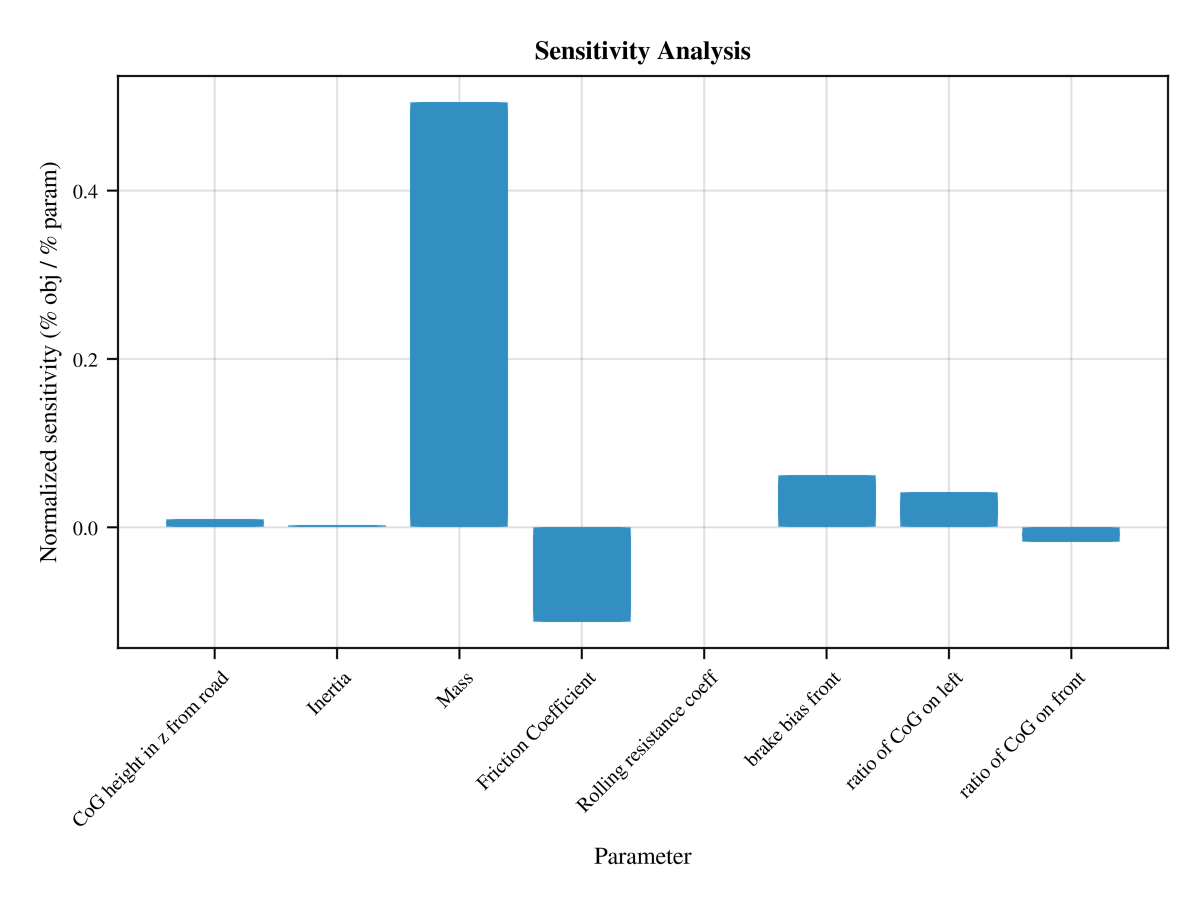
\includegraphics[width=1\textwidth]{../sync/sensitivity.png}}
	\caption{Node-interval ODE error for power-test case.}
	\label{fig:sensitivity}
\end{figure}

\section{Implemented nonlinear programming solvers}
Julia with JuMP offer high level interface which allows switching NLP solvers on single line. I have used Ipopt, MadNLP and Uno solver with preset filtersqp. Unfortunately the Uno solver was getting stuck, therefore it is not cosidered in this thesis.

Ipopt has built in Hessian aproximation strategy, in benchmark it proved to be inferior to automatic differentiation. Figure \ref{fig:nlp_flowchart_chosen} shows which solving methods were implemented and tested.
\begin{figure}[H]
\centering
\begin{tikzpicture}[
  >={Latex[length=2mm]},
  node distance=0.6cm and 0.15cm,
  every node/.style={font=\small, align=center},
  box/.style={draw, minimum height=0.7cm, inner sep=3pt},
  problem/.style={box},
  branch/.style={box, font=\small, text width=2.2cm},
  stagebox/.style={box, text width=2.6cm, font=\footnotesize},
  deriv/.style={box, text width=1.4cm, font=\footnotesize},
  terminal/.style={box, line width=1pt},
  chosen/.style={fill=green!30}
]

\node[problem] (nlp) {Transcribed nonlinear programming problem};

\node[branch, below=0.75cm of nlp, xshift=-1.5cm] (sqp) {Sequential\\Quadratic\\Programming};
\node[branch, below=0.75cm of nlp, xshift=1.5cm, chosen] (ipm) {Interior\\Point\\Methods};

\node[problem, below=3cm of nlp] (need) {Compute derivatives};

\node[deriv, below=1cm of need] (fd) {Finite\\differences};
\node[deriv, left=of fd]  (sym)  {Symbolic};
\node[deriv, left=of sym] (anal) {Analytic};
\node[deriv, right=of fd, chosen] (ad)   {Automatic\\diff.};
\node[deriv, right=of ad, chosen] (qn)   {Quasi-\\Newton\\methods};

\node[terminal, below=3cm of need] (newton) {Assemble linear system\\\textbf{Newton step}};

\draw[->] (nlp) -- (sqp);
\draw[->, very thick, green!60!black] (nlp) -- (ipm);
\draw[->] (sqp) -- (need);
\draw[->, very thick, green!60!black] (ipm) -- (need);

\draw[->] (need) -- (anal);
\draw[->] (need) -- (sym);
\draw[->] (need) -- (fd);
\draw[->, very thick, green!60!black] (need) -- (ad);
\draw[->, very thick, green!60!black] (need) -- (qn);

\draw[->] (anal) -- (newton);
\draw[->] (sym)  -- (newton);
\draw[->] (fd)   -- (newton);
\draw[->, very thick, green!60!black] (ad)   -- (newton);
\draw[->, very thick, green!60!black] (qn)   -- (newton);

\end{tikzpicture}
\caption{NLP solution flow with the methods used in this thesis highlighted in green}
\label{fig:nlp_flowchart_chosen}
\end{figure}
\section{Implementation of mesh refinement}
I have implemented p and h method for mesh refinement. Error calculation is implemented using comparing the result of interpolated value at the and of segment and the result of simulation using Rodas4() solver.

To calculate the error at the end of each segment, the interpolated controls and intial states are plugged into Rodas4 IVP solver. Then this result is compared to the states from transcription method. If error between states in absolute vlaue is larger than user defined threshold, the segment is halved. This one of the simpler estimators of discretization error.


Figure \ref{fig:power_node_controls} shows that
error along track is not distributed equaly. Error is localised around areas
with large jump in controls. These areas need finer sampling. P methods cannot
focus these specific points directly, they focus entire trajectory.

The errors are concentrated around the discontinuity of controls, where the
behaviour of the vehicle is more complex/ requiring high order or finer
approximation see Figure \ref{fig:power_node_controls}. Time optimal control of car around track has many discontinuities and therefore p methods are not a good fit for this use.


\begin{figure}[H]
    \centering
    \makebox[\textwidth][c]{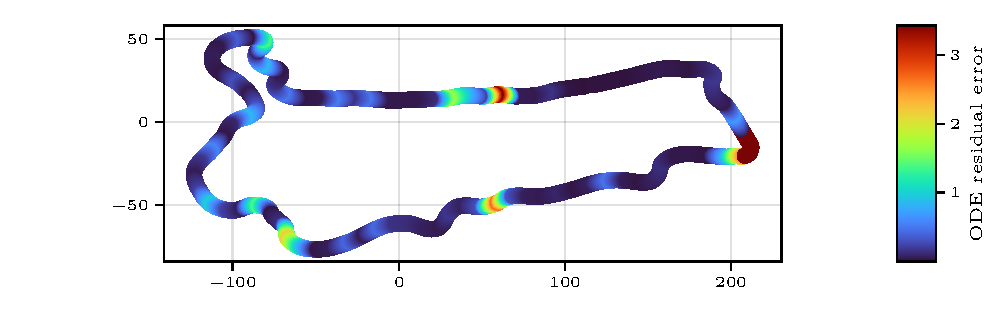
\includegraphics[width=1\textwidth]{../sync/thesisImages/mesh_refinement_fscz_error_iter0.pdf}}
    \caption{Node-interval ODE error for power-test case.}
    \label{fig:power_node_controls}
\end{figure}

\begin{figure}[H]
    \centering
    \makebox[\textwidth][c]{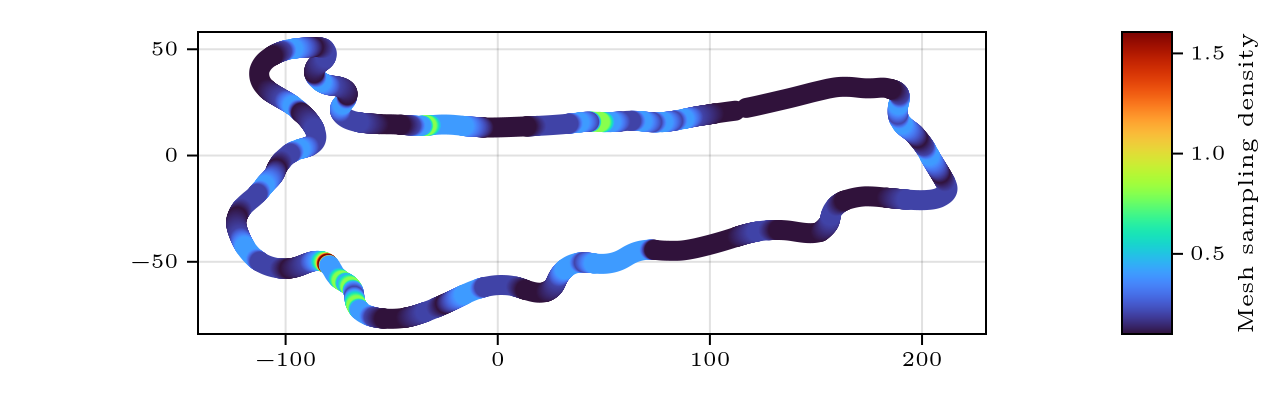
\includegraphics[width=1\textwidth]{../sync/thesisImages/mesh_refinement_fscz_density_iter10.png}}
    \caption{Node-interval ODE error for power-test case.}
    \label{fig:power_node_controls}
\end{figure}



\begin{figure}[H]
    \centering
    \makebox[\textwidth][c]{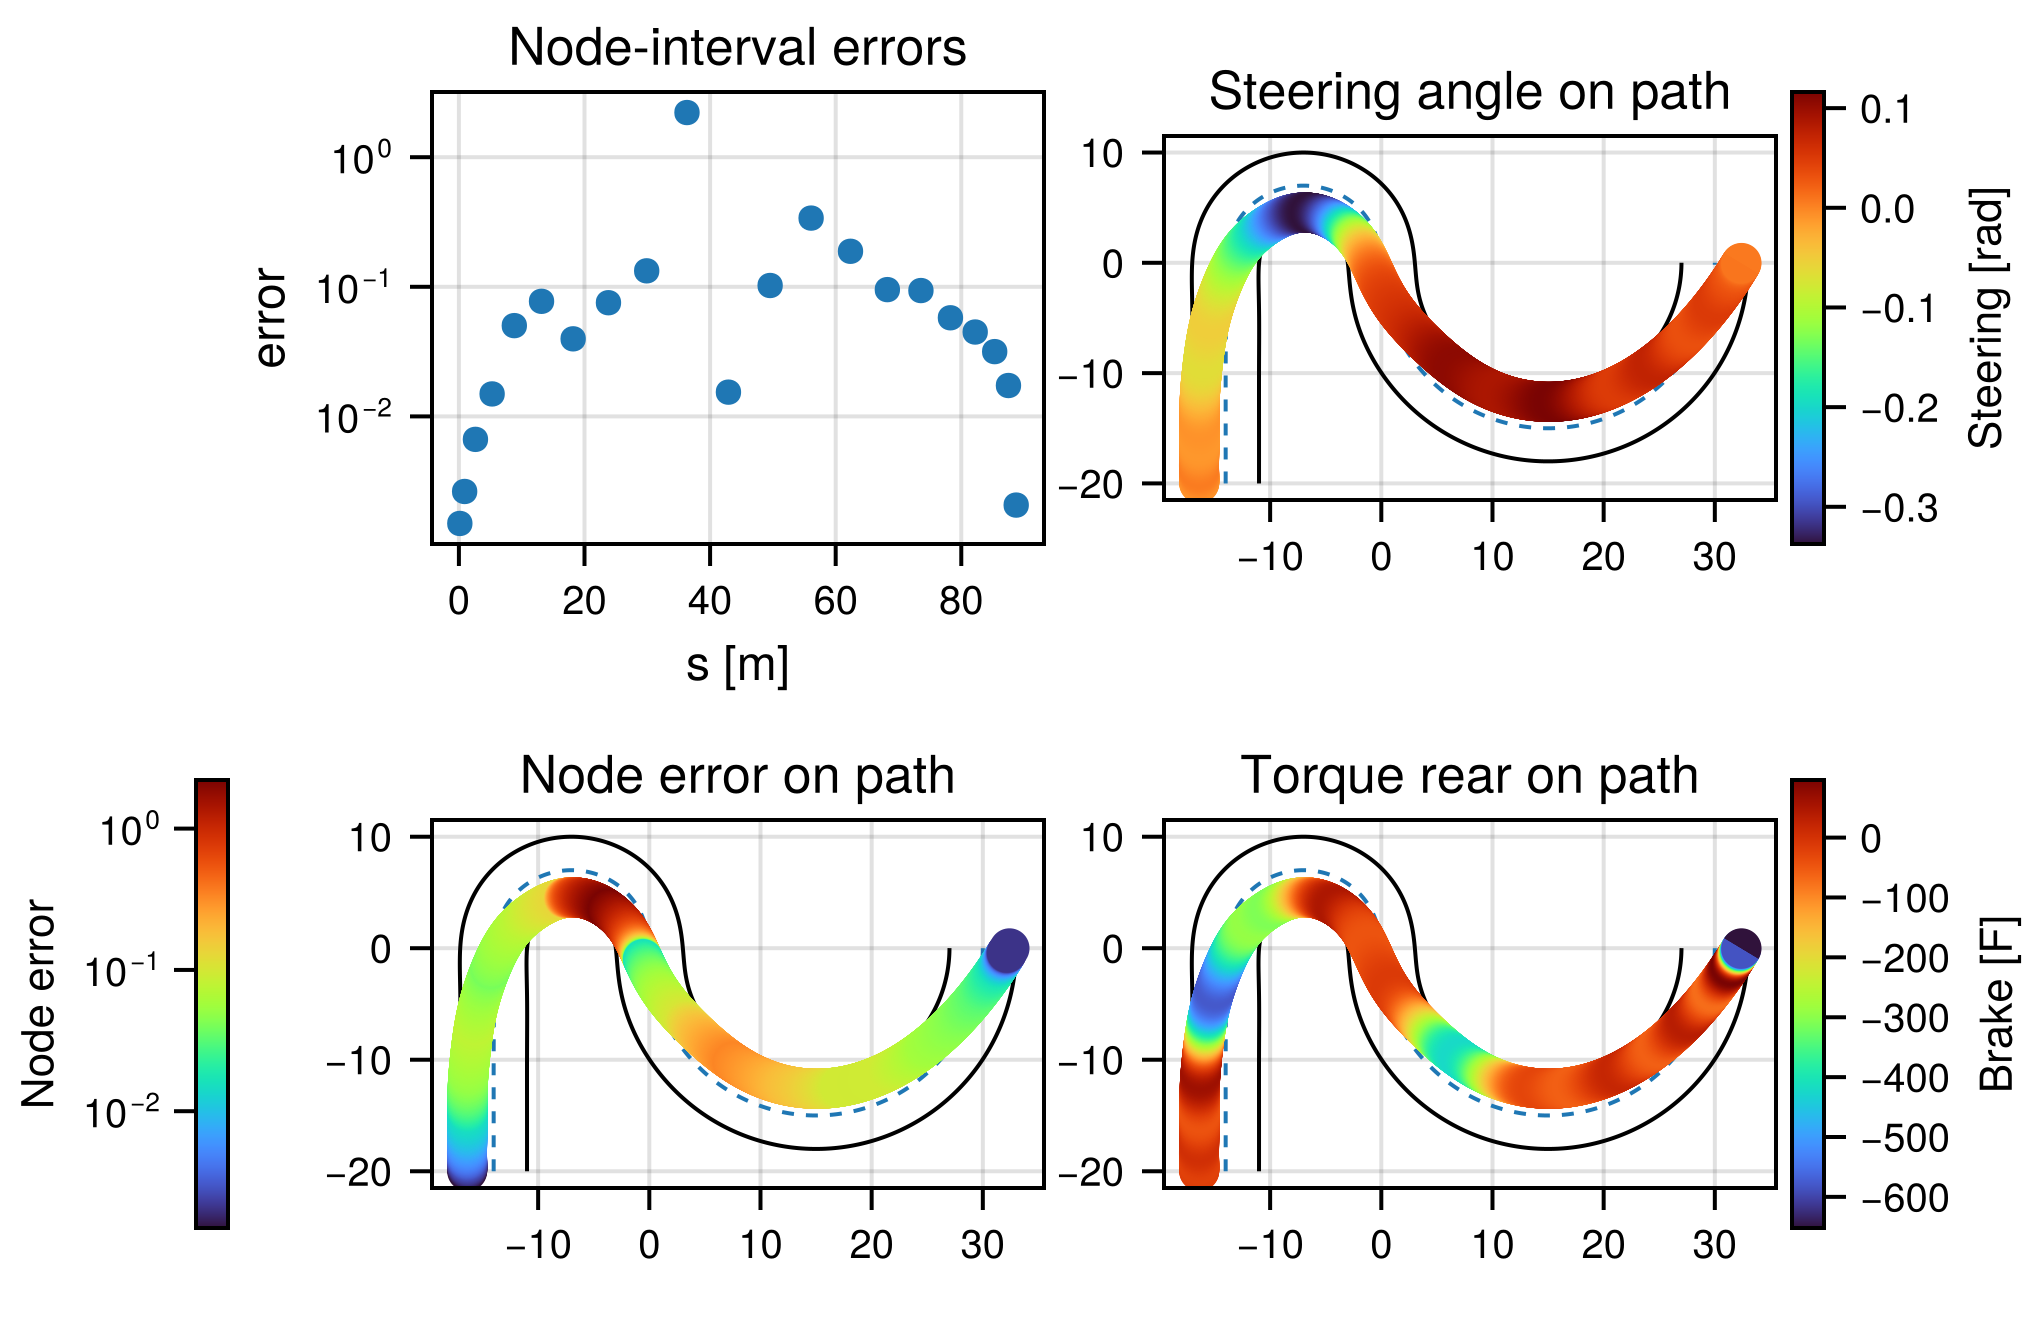
\includegraphics[width=1\textwidth]{../sync/p_methodplots/power_summary2x2.png}}
    \caption{Node-interval ODE error for power-test case.}
    \label{fig:power_node_controls}
\end{figure}



\begin{figure}[H]
\centering
\begin{tikzpicture}[
  >={Latex[length=2mm]},
  node distance=0.7cm and 0.35cm,
  method/.style={draw, text width=2.4cm, minimum height=0.9cm, align=center, font=\small, inner sep=3pt},
  layer/.style={draw, minimum height=0.8cm, inner sep=4pt, align=center, font=\normalsize\bfseries},
  chosen/.style={fill=green!30}
]

\node[method, chosen]      (p)   {$p$-refinement\\(raise polynomial degree)};
\node[method, chosen, right=of p]  (h)   {$h$-refinement\\(subdivide segments)};
\node[method, right=of h]  (hp)  {$hp$-refinement\\(p first, then h)};
\node[method, right=of hp] (ph)  {$ph$-refinement\\(h first, then p)};

\node[layer, above=1cm of $(p.north)!0.5!(ph.north)$] (mesh)
  {Mesh refinement strategy};

\draw[->, very thick, green!60!black] (mesh.south) -- (p.north);
\draw[->, very thick, green!60!black] (mesh.south) -- (h.north);
\draw[->] (mesh.south) -- (hp.north);
\draw[->] (mesh.south) -- (ph.north);

\end{tikzpicture}
\caption{Mesh refinement layer with the strategies implemented in this thesis highlighted in green}
\label{fig:mesh_refinement_chosen}
\end{figure}

\section{Implementation of collocation methods}
\begin{figure}[H]
\centering
\begin{tikzpicture}[
  >={Latex[length=2mm]},
  node distance=0.55cm and 0.18cm,
  basis/.style={draw, text width=1.4cm, minimum height=0.8cm, align=center, font=\scriptsize, inner sep=2pt},
  scheme/.style={draw, text width=3.2cm, minimum height=0.8cm, align=center, font=\small, inner sep=3pt},
  form/.style={draw, text width=1.25cm, minimum height=0.6cm, align=center, font=\scriptsize, inner sep=2pt},
  layer/.style={draw, minimum height=0.8cm, inner sep=4pt, align=center, font=\normalsize\bfseries},
  chosen/.style={fill=green!30}
]

\node[basis]                    (cheb) {Chebyshev\\I \& II};
\node[basis, right=of cheb]     (her)  {Hermite};
\node[basis, right=of her]      (lag)  {Laguerre};
\node[basis, right=of lag, chosen] (leg)  {Legendre};
\node[basis, right=of leg]      (alag) {Assoc.\\Laguerre};
\node[basis, right=of alag]     (geg)  {Gegenbauer};
\node[basis, right=of geg]      (jac)  {Jacobi};

\node[layer, above=1cm of $(cheb.north)!0.5!(jac.north)$] (trans)
  {Transcription:\\orthogonal polynomial basis};

\foreach \n in {cheb,her,lag,alag,geg,jac}
  \draw[->] (trans.south) -- (\n.north);
\draw[->, very thick, green!60!black] (trans.south) -- (leg.north);

\node[scheme, chosen, below=1.8cm of leg] (lgr) {Legendre--Gauss--Radau\\(LGR) Quadrature};
\node[scheme, chosen, left=of lgr]  (lg)  {Legendre--Gauss\\(LG) Quadrature};
\node[scheme, chosen, right=of lgr] (lgl) {Legendre--Gauss--Lobatto\\(LGL) Quadrature};

\draw[->, very thick, green!60!black] (leg.south) -- (lg.north);
\draw[->, very thick, green!60!black] (leg.south) -- (lgr.north);
\draw[->, very thick, green!60!black] (leg.south) -- (lgl.north);

\foreach \n in {cheb,her,lag,alag,geg,jac}
  \node[font=\Large, below=0.35cm of \n] {$\vdots$};

\node[form, below=0.8cm of lg, xshift=-0.85cm]         (lg-int)  {Integral};
\node[form, chosen, below=0.8cm of lg, xshift=0.85cm]  (lg-diff) {Differ.};
\draw[->] (lg.south) -- (lg-int.north);
\draw[->, very thick, green!60!black] (lg.south) -- (lg-diff.north);

\node[form, below=0.8cm of lgr, xshift=-0.85cm]         (lgr-int)  {Integral};
\node[form, chosen, below=0.8cm of lgr, xshift=0.85cm]  (lgr-diff) {Differ.};
\draw[->] (lgr.south) -- (lgr-int.north);
\draw[->, very thick, green!60!black] (lgr.south) -- (lgr-diff.north);

\node[form, chosen, below=0.8cm of lgl, xshift=-0.85cm] (lgl-int)  {Integral};
\node[form, below=0.8cm of lgl, xshift=0.85cm]          (lgl-diff) {Differ.};
\draw[->, very thick, green!60!black] (lgl.south) -- (lgl-int.north);
\draw[->] (lgl.south) -- (lgl-diff.north);

\end{tikzpicture}
\caption{Transcription layer with the methods used in this thesis highlighted in green}
\label{fig:transcription_chosen}
\end{figure}


\section{My collocation}
my mesh refinbment error calc + my methods implemented

\section{my mesh refinment}
ode error

\section{My car models}
PUT CAR MODELS HERE
\subsection{singletrack}
\subsection{Formula Student twintrack}
\subsection{FormulaE}
\subsection{Bus}
%\subsection{my tires}

%\subsection{my suspensions}

\section{Benchmark tracks}
The following tracks are used in the benchmark in
Section~\ref{sec:benchmark}. They cover real Formula Student layouts
(FSCZ, FSG), a Formula~E street circuit (Berlin) and two synthetic
geometries (DoubleTurn, FigureEight).

\begin{figure}[H]
    \centering
    \begin{subfigure}[t]{0.48\textwidth}
        \centering
        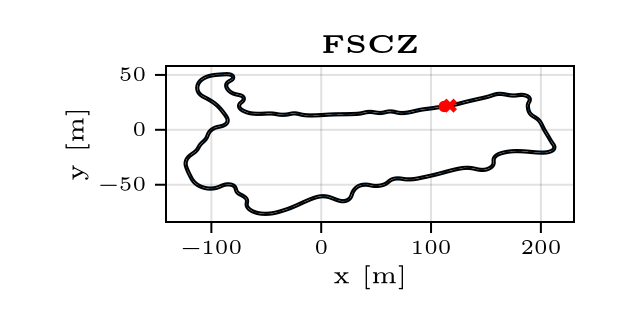
\includegraphics[width=\linewidth]{../sync/thesisImages/benchmark_track_FSCZ.png}
        \caption{Formula Student Czech track}
        \label{fig:track_fscz}
    \end{subfigure}\hfill
    \begin{subfigure}[t]{0.48\textwidth}
        \centering
        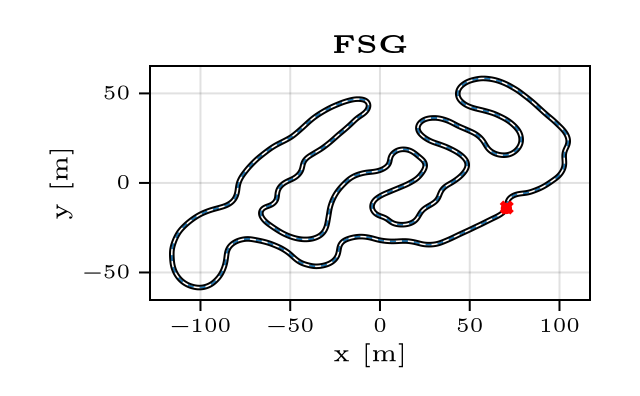
\includegraphics[width=\linewidth]{../sync/thesisImages/benchmark_track_FSG.png}
        \caption{Formula Student Germany track}
        \label{fig:track_fsg}
    \end{subfigure}

    \vspace{0.5em}
    \begin{subfigure}[t]{0.48\textwidth}
        \centering
        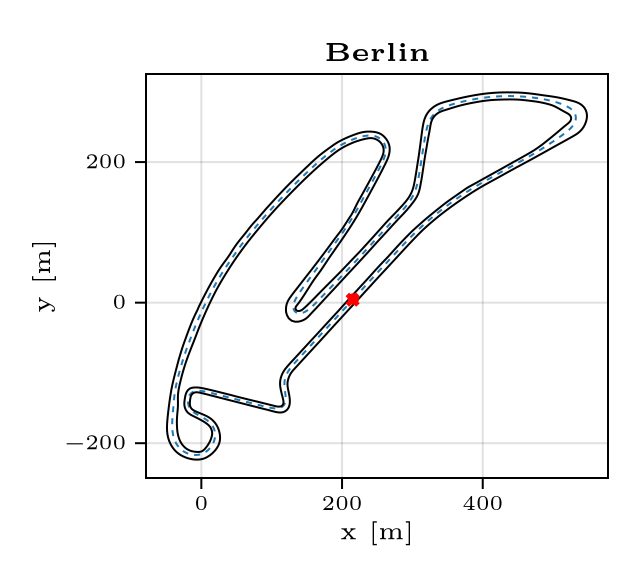
\includegraphics[width=\linewidth]{../sync/thesisImages/benchmark_track_Berlin.png}
        \caption{Berlin (Formula~E)}
        \label{fig:track_berlin}
    \end{subfigure}\hfill
    \begin{subfigure}[t]{0.48\textwidth}
        \centering
        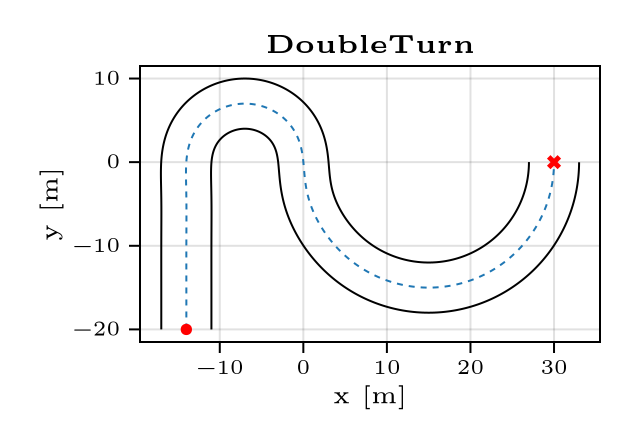
\includegraphics[width=\linewidth]{../sync/thesisImages/benchmark_track_DoubleTurn.png}
        \caption{DoubleTurn}
        \label{fig:track_doubleturn}
    \end{subfigure}

    \vspace{0.5em}
    \begin{subfigure}[t]{0.48\textwidth}
        \centering
        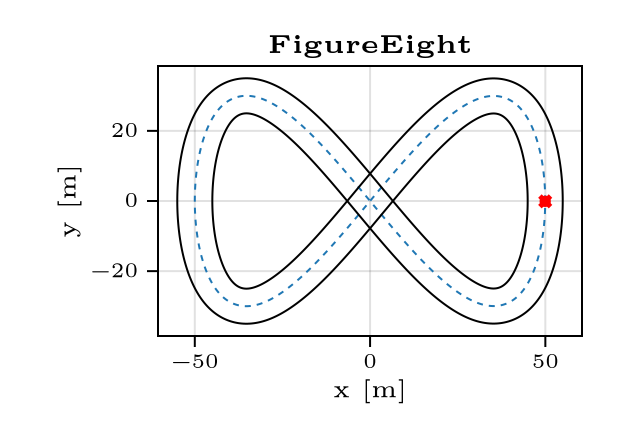
\includegraphics[width=\linewidth]{../sync/thesisImages/benchmark_track_FigureEight.png}
        \caption{FigureEight}
        \label{fig:track_figureeight}
    \end{subfigure}
    \caption{Tracks used in the solver/transcription benchmark.}
    \label{fig:benchmark_tracks}
\end{figure}

\section{Actual constriants, exampleconstraints like cannot leave road}

\part{results}
\chapter{comparison of methods}
Performace of NLP solvers and frameworks is often tested on benchmark problems. like CUTEst \cite{gouldCUTEstConstrainedUnconstrained2014} dataset?
Tests were performed on Ryzen 9 9950X and MadNLP ran on Nvidia RTX
5070. Important caveat is that IPOPT has many (probably too many) options which can be adjusted, and that is true for all solvers. Some of differences in this benchmark may be due to sub optimal setup of the solver.
\begin{table}[!ht]
\centering
{\footnotesize
\begin{longtable}{|r|r|r|r|r|r|r|r|r|}
  \hline
  \textbf{transcription} & \textbf{runs} & \textbf{ok} & \textbf{fail} & \textbf{rate} & \textbf{mean\_s} & \textbf{med\_s} & \textbf{min\_s} & \textbf{max\_s} \\
  \hline
  Legendre & 14 & 14 & 0 & 100.0000 & 167.1341 & 25.1476 & 0.8392 & 1688.6196 \\
  Lobatto IIIA & 14 & 14 & 0 & 100.0000 & 58.1844 & 16.6429 & 0.3494 & 546.0076 \\
  Radau & 14 & 14 & 0 & 100.0000 & 183.1201 & 14.4853 & 0.7666 & 2272.8209 \\
  \hline
\end{longtable}
}

\caption{Benchmark summary statistics by transcription variant.}
\label{tab:benchmark-summary}
\end{table}



\begin{table}[!ht]
\centering
{\footnotesize
\begin{longtable}{|r|r|r|r|r|r|r|}
  \hline
  \textbf{track} & \textbf{car} & \textbf{transcription} & \textbf{ok} & \textbf{status} & \textbf{time\_s} & \textbf{obj} \\
  \hline
  FSCZ & singletrack & Radau & yes & solved & 9.6201 & 47.1377 \\
  FSCZ & singletrack & Legendre & yes & solved & 26.7235 & 47.2675 \\
  FSCZ & singletrack & Lobatto IIIA & yes & solved & 17.8552 & 47.5837 \\
  FSCZ & twintrack & Radau & yes & solved & 29.3340 & 53.1709 \\
  FSCZ & twintrack & Legendre & yes & solved & 61.1884 & 53.4512 \\
  FSCZ & twintrack & Lobatto IIIA & yes & solved & 25.6206 & 53.9954 \\
  Berlin & singletrack & Radau & yes & solved & 22.0242 & 79.4397 \\
  Berlin & singletrack & Legendre & yes & solved & 23.5717 & 79.4492 \\
  Berlin & singletrack & Lobatto IIIA & yes & solved & 52.4490 & 79.4002 \\
  Berlin & twintrack & Radau & yes & solved & 73.7309 & 77.7238 \\
  Berlin & twintrack & Legendre & yes & solved & 46.3706 & 78.0661 \\
  Berlin & twintrack & Lobatto IIIA & yes & solved & 32.2219 & 77.7762 \\
  Berlin & formula & Radau & yes & solved & 72.6660 & 87.9109 \\
  Berlin & formula & Legendre & yes & solved & 407.0615 & 88.9009 \\
  Berlin & formula & Lobatto IIIA & yes & solved & 63.9919 & 87.9114 \\
  Berlin & bus & Radau & yes & solved & 2272.8209 & 106.6878 \\
  Berlin & bus & Legendre & yes & solved & 1688.6196 & 106.7405 \\
  Berlin & bus & Lobatto IIIA & yes & solved & 546.0076 & 106.1627 \\
  FSG & singletrack & Radau & yes & solved & 11.4388 & 53.8713 \\
  FSG & singletrack & Legendre & yes & solved & 28.6402 & 53.9862 \\
  FSG & singletrack & Lobatto IIIA & yes & solved & 15.4307 & 53.4303 \\
  FSG & twintrack & Radau & yes & solved & 46.4263 & 64.6331 \\
  FSG & twintrack & Legendre & yes & solved & 36.2408 & 64.7986 \\
  FSG & twintrack & Lobatto IIIA & yes & solved & 48.9636 & 64.2024 \\
  DoubleTurn & singletrack & Radau & yes & solved & 1.2873 & 5.6450 \\
  DoubleTurn & singletrack & Legendre & yes & solved & 0.8392 & 5.6384 \\
  DoubleTurn & singletrack & Lobatto IIIA & yes & solved & 0.3494 & 5.6922 \\
  DoubleTurn & twintrack & Radau & yes & solved & 0.7666 & 6.5474 \\
  DoubleTurn & twintrack & Legendre & yes & solved & 0.8690 & 6.5527 \\
  DoubleTurn & twintrack & Lobatto IIIA & yes & solved & 0.6170 & 6.7016 \\
  DoubleTurn & bus & Radau & yes & solved & 1.6908 & 8.9032 \\
  DoubleTurn & bus & Legendre & yes & solved & 1.4636 & 8.9150 \\
  DoubleTurn & bus & Lobatto IIIA & yes & solved & 2.0459 & 8.8830 \\
  FigureEight & singletrack & Radau & yes & solved & 1.1828 & 14.9425 \\
  FigureEight & singletrack & Legendre & yes & solved & 2.0092 & 14.9482 \\
  FigureEight & singletrack & Lobatto IIIA & yes & solved & 2.8800 & 14.8949 \\
  FigureEight & twintrack & Radau & yes & solved & 3.1612 & 16.6011 \\
  FigureEight & twintrack & Legendre & yes & solved & 7.5868 & 16.6084 \\
  FigureEight & twintrack & Lobatto IIIA & yes & solved & 1.9091 & 16.6481 \\
  FigureEight & bus & Radau & yes & solved & 17.5317 & 22.8455 \\
  FigureEight & bus & Legendre & yes & solved & 8.6937 & 22.8542 \\
  FigureEight & bus & Lobatto IIIA & yes & solved & 4.2393 & 22.4779 \\
  \hline
\end{longtable}
}

\caption{Benchmark results by track, vehicle model, and transcription variant.}
\label{tab:benchmark-results}
\end{table}




\begin{table}[!ht]
\centering
{\footnotesize
\begin{longtable}{|r|r|r|r|r|r|r|r|r|}
  \hline
  \textbf{linear solver} & \textbf{runs} & \textbf{ok} & \textbf{fail} & \textbf{rate} & \textbf{mean\_s} & \textbf{med\_s} & \textbf{min\_s} & \textbf{max\_s} \\
  \hline
  ma27 & 14 & 14 & 0 & 100.0000 & 261.8886 & 14.3300 & 0.3385 & 3390.5082 \\
  ma57 & 14 & 14 & 0 & 100.0000 & 80.8659 & 14.0413 & 0.7563 & 839.6873 \\
  ma97 & 14 & 13 & 1 & 92.8571 & 22.9438 & 12.2251 & 0.3456 & 80.9731 \\
  mumps & 14 & 14 & 0 & 100.0000 & 182.9820 & 14.3890 & 0.3590 & 2264.3630 \\
  \hline
\end{longtable}
}

\caption{Linear solver benchmark summary statistics.}
\label{tab:linsolver-summary}
\end{table}



\begin{table}[!ht]
\centering
{\footnotesize
\begin{longtable}{|r|r|r|r|r|r|r|}
  \hline
  \textbf{track} & \textbf{car} & \textbf{linear solver} & \textbf{ok} & \textbf{status} & \textbf{time\_s} & \textbf{obj} \\
  \hline
  FSCZ & singletrack & mumps & yes & solved & 9.5894 & 47.1377 \\
  FSCZ & singletrack & ma57 & yes & solved & 11.3044 & 47.1377 \\
  FSCZ & singletrack & ma27 & yes & solved & 9.3451 & 47.1377 \\
  FSCZ & singletrack & ma97 & yes & solved & 10.5403 & 47.1377 \\
  FSCZ & twintrack & mumps & yes & solved & 29.3824 & 53.1709 \\
  FSCZ & twintrack & ma57 & yes & solved & 26.9544 & 53.1709 \\
  FSCZ & twintrack & ma27 & yes & solved & 28.0511 & 53.1709 \\
  FSCZ & twintrack & ma97 & yes & solved & 26.3581 & 53.1709 \\
  Berlin & singletrack & mumps & yes & solved & 25.9843 & 79.4397 \\
  Berlin & singletrack & ma57 & yes & solved & 18.4504 & 79.4397 \\
  Berlin & singletrack & ma27 & yes & solved & 19.2238 & 79.4397 \\
  Berlin & singletrack & ma97 & yes & solved & 27.0323 & 79.4397 \\
  Berlin & twintrack & mumps & yes & solved & 75.4742 & 77.7238 \\
  Berlin & twintrack & ma57 & yes & solved & 58.6173 & 77.7238 \\
  Berlin & twintrack & ma27 & yes & solved & 67.6959 & 77.7238 \\
  Berlin & twintrack & ma97 & yes & solved & 80.9731 & 77.7238 \\
  Berlin & formula & mumps & yes & solved & 73.7649 & 87.9109 \\
  Berlin & formula & ma57 & yes & solved & 99.8552 & 87.9109 \\
  Berlin & formula & ma27 & yes & solved & 72.8937 & 87.9109 \\
  Berlin & formula & ma97 & yes & solved & 78.1892 & 87.9103 \\
  Berlin & bus & mumps & yes & solved & 2264.3630 & 106.6878 \\
  Berlin & bus & ma57 & yes & solved & 839.6873 & 106.6882 \\
  Berlin & bus & ma27 & yes & solved & 3390.5082 & 106.7080 \\
  Berlin & bus & ma97 & no & iteration limit & 605.6959 & NaN \\
  FSG & singletrack & mumps & yes & solved & 11.5927 & 53.8713 \\
  FSG & singletrack & ma57 & yes & solved & 12.5714 & 53.8713 \\
  FSG & singletrack & ma27 & yes & solved & 12.9429 & 53.8713 \\
  FSG & singletrack & ma97 & yes & solved & 12.2251 & 53.8713 \\
  FSG & twintrack & mumps & yes & solved & 47.1838 & 64.6331 \\
  FSG & twintrack & ma57 & yes & solved & 41.5523 & 64.6331 \\
  FSG & twintrack & ma27 & yes & solved & 44.1811 & 64.6331 \\
  FSG & twintrack & ma97 & yes & solved & 40.6957 & 64.6380 \\
  DoubleTurn & singletrack & mumps & yes & solved & 0.3590 & 5.6450 \\
  DoubleTurn & singletrack & ma57 & yes & solved & 1.3340 & 5.6450 \\
  DoubleTurn & singletrack & ma27 & yes & solved & 0.3385 & 5.6450 \\
  DoubleTurn & singletrack & ma97 & yes & solved & 0.3456 & 5.6450 \\
  DoubleTurn & twintrack & mumps & yes & solved & 0.6577 & 6.5474 \\
  DoubleTurn & twintrack & ma57 & yes & solved & 0.8025 & 6.5474 \\
  DoubleTurn & twintrack & ma27 & yes & solved & 0.6423 & 6.5474 \\
  DoubleTurn & twintrack & ma97 & yes & solved & 0.5053 & 6.5488 \\
  DoubleTurn & bus & mumps & yes & solved & 0.9267 & 8.9032 \\
  DoubleTurn & bus & ma57 & yes & solved & 0.7563 & 8.9032 \\
  DoubleTurn & bus & ma27 & yes & solved & 0.8304 & 8.9032 \\
  DoubleTurn & bus & ma97 & yes & solved & 0.7686 & 8.9032 \\
  FigureEight & singletrack & mumps & yes & solved & 1.2690 & 14.9425 \\
  FigureEight & singletrack & ma57 & yes & solved & 1.9768 & 14.9425 \\
  FigureEight & singletrack & ma27 & yes & solved & 1.2471 & 14.9425 \\
  FigureEight & singletrack & ma97 & yes & solved & 1.0779 & 14.9425 \\
  FigureEight & twintrack & mumps & yes & solved & 4.0156 & 16.6011 \\
  FigureEight & twintrack & ma57 & yes & solved & 2.7487 & 16.6011 \\
  FigureEight & twintrack & ma27 & yes & solved & 2.8235 & 16.6011 \\
  FigureEight & twintrack & ma97 & yes & solved & 3.7290 & 16.6011 \\
  FigureEight & bus & mumps & yes & solved & 17.1854 & 22.8455 \\
  FigureEight & bus & ma57 & yes & solved & 15.5112 & 22.8455 \\
  FigureEight & bus & ma27 & yes & solved & 15.7170 & 22.8455 \\
  FigureEight & bus & ma97 & yes & solved & 15.8290 & 22.8455 \\
  \hline
\end{longtable}
}

\caption{Linear solver benchmark results by track, vehicle model, and transcription variant.}
\label{tab:linsolver-results}
\end{table}



\begin{table}[!ht]
\centering
{\footnotesize
\begin{longtable}{|r|r|r|r|r|r|r|r|r|}
  \hline
  \textbf{NLP solver} & \textbf{runs} & \textbf{ok} & \textbf{fail} & \textbf{rate} & \textbf{mean\_s} & \textbf{med\_s} & \textbf{min\_s} & \textbf{max\_s} \\
  \hline
  ipopt-mumps & 14 & 14 & 0 & 100.0000 & 194.9796 & 14.2172 & 0.3935 & 2443.6578 \\
  madnlp-cpu & 14 & 13 & 1 & 92.8571 & 23.3577 & 14.0445 & 0.3068 & 94.4898 \\
  madnlp-gpu & 14 & 13 & 1 & 92.8571 & 30.0594 & 14.8362 & 0.6094 & 137.7783 \\
  \hline
\end{longtable}
}

\caption{NLP solver / backend benchmark summary statistics (IPOPT-MUMPS, MadNLP-CPU, MadNLP-GPU).}
\label{tab:backend-summary}
\end{table}



\begin{table}[!ht]
\centering
{\footnotesize
\begin{longtable}{|r|r|r|r|r|r|r|}
  \hline
  \textbf{track} & \textbf{car} & \textbf{NLP solver} & \textbf{ok} & \textbf{status} & \textbf{time\_s} & \textbf{obj} \\
  \hline
  FSCZ & singletrack & ipopt-mumps & yes & solved & 10.4205 & 47.1377 \\
  FSCZ & singletrack & madnlp-cpu & yes & solved & 18.3293 & 47.1377 \\
  FSCZ & singletrack & madnlp-gpu & yes & solved & 66.7619 & 47.1363 \\
  FSCZ & twintrack & ipopt-mumps & yes & solved & 29.6126 & 53.1709 \\
  FSCZ & twintrack & madnlp-cpu & yes & solved & 31.7456 & 53.1709 \\
  FSCZ & twintrack & madnlp-gpu & yes & solved & 60.5383 & 53.2287 \\
  Berlin & singletrack & ipopt-mumps & yes & solved & 16.7130 & 79.4397 \\
  Berlin & singletrack & madnlp-cpu & yes & solved & 14.0445 & 79.4397 \\
  Berlin & singletrack & madnlp-gpu & yes & solved & 14.8362 & 79.4358 \\
  Berlin & twintrack & ipopt-mumps & yes & solved & 72.1841 & 77.7238 \\
  Berlin & twintrack & madnlp-cpu & yes & solved & 94.4898 & 77.7237 \\
  Berlin & twintrack & madnlp-gpu & yes & solved & 23.4224 & 77.7201 \\
  Berlin & formula & ipopt-mumps & yes & solved & 71.9810 & 87.9109 \\
  Berlin & formula & madnlp-cpu & yes & solved & 81.3535 & 87.9111 \\
  Berlin & formula & madnlp-gpu & yes & almost locally solved & 137.7783 & 87.9093 \\
  Berlin & bus & ipopt-mumps & yes & solved & 2443.6578 & 106.6937 \\
  Berlin & bus & madnlp-cpu & no & iteration limit & 1178.0533 & NaN \\
  Berlin & bus & madnlp-gpu & no & iteration limit & 4431.9955 & NaN \\
  FSG & singletrack & ipopt-mumps & yes & solved & 11.7215 & 53.8713 \\
  FSG & singletrack & madnlp-cpu & yes & solved & 12.8528 & 53.8713 \\
  FSG & singletrack & madnlp-gpu & yes & solved & 12.2274 & 53.8696 \\
  FSG & twintrack & ipopt-mumps & yes & solved & 47.4247 & 64.6331 \\
  FSG & twintrack & madnlp-cpu & yes & solved & 29.7381 & 64.5931 \\
  FSG & twintrack & madnlp-gpu & yes & solved & 29.5928 & 64.5912 \\
  DoubleTurn & singletrack & ipopt-mumps & yes & solved & 0.3935 & 5.6450 \\
  DoubleTurn & singletrack & madnlp-cpu & yes & solved & 0.3068 & 5.6450 \\
  DoubleTurn & singletrack & madnlp-gpu & yes & solved & 0.6094 & 5.6449 \\
  DoubleTurn & twintrack & ipopt-mumps & yes & solved & 0.6312 & 6.5474 \\
  DoubleTurn & twintrack & madnlp-cpu & yes & solved & 0.7809 & 6.5488 \\
  DoubleTurn & twintrack & madnlp-gpu & yes & solved & 0.7918 & 6.5487 \\
  DoubleTurn & bus & ipopt-mumps & yes & solved & 1.8919 & 8.9032 \\
  DoubleTurn & bus & madnlp-cpu & yes & solved & 0.7989 & 8.9032 \\
  DoubleTurn & bus & madnlp-gpu & yes & solved & 1.4556 & 8.9031 \\
  FigureEight & singletrack & ipopt-mumps & yes & solved & 1.4011 & 14.9425 \\
  FigureEight & singletrack & madnlp-cpu & yes & solved & 1.2097 & 14.9425 \\
  FigureEight & singletrack & madnlp-gpu & yes & solved & 1.2459 & 14.9419 \\
  FigureEight & twintrack & ipopt-mumps & yes & solved & 4.1659 & 16.6011 \\
  FigureEight & twintrack & madnlp-cpu & yes & solved & 2.4902 & 16.6011 \\
  FigureEight & twintrack & madnlp-gpu & yes & solved & 2.6734 & 16.5974 \\
  FigureEight & bus & ipopt-mumps & yes & solved & 17.5150 & 22.8455 \\
  FigureEight & bus & madnlp-cpu & yes & solved & 15.5101 & 22.9008 \\
  FigureEight & bus & madnlp-gpu & yes & solved & 38.8391 & 22.9871 \\
  \hline
\end{longtable}
}

\caption{NLP solver / backend benchmark results by track, vehicle model, and transcription variant.}
\label{tab:backend-results}
\end{table}

\begin{table}[!ht]
\centering
{\footnotesize
\begin{longtable}{|r|r|r|r|r|r|r|r|r|}
  \hline
  \textbf{hessian mode} & \textbf{runs} & \textbf{ok} & \textbf{fail} & \textbf{rate} & \textbf{mean\_s} & \textbf{med\_s} & \textbf{min\_s} & \textbf{max\_s} \\
  \hline
  ipopt-exact & 14 & 14 & 0 & 100.0000 & 196.4979 & 14.3078 & 0.3420 & 2459.4467 \\
  ipopt-lbfgs & 14 & 7 & 7 & 50.0000 & 9.9792 & 7.3379 & 0.4952 & 25.2870 \\
  \hline
\end{longtable}
}

\caption{Hessian approximation benchmark summary statistics (exact vs.\ limited-memory quasi-Newton).}
\label{tab:hessian-summary}
\end{table}

\begin{table}[!ht]
\centering
{\footnotesize
\begin{longtable}{|r|r|r|r|r|r|r|}
  \hline
  \textbf{track} & \textbf{car} & \textbf{hessian mode} & \textbf{ok} & \textbf{status} & \textbf{time\_s} & \textbf{obj} \\
  \hline
  FSCZ & singletrack & ipopt-exact & yes & solved & 10.6736 & 47.1377 \\
  FSCZ & singletrack & ipopt-lbfgs & yes & almost locally solved & 16.1547 & 47.1377 \\
  FSCZ & twintrack & ipopt-exact & yes & solved & 30.6336 & 53.1709 \\
  FSCZ & twintrack & ipopt-lbfgs & no & iteration limit & 315.6241 & NaN \\
  Berlin & singletrack & ipopt-exact & yes & solved & 17.1804 & 79.4397 \\
  Berlin & singletrack & ipopt-lbfgs & yes & almost locally solved & 25.2870 & 79.4397 \\
  Berlin & twintrack & ipopt-exact & yes & solved & 71.7344 & 77.7238 \\
  Berlin & twintrack & ipopt-lbfgs & no & iteration limit & 1269.5613 & NaN \\
  Berlin & formula & ipopt-exact & yes & solved & 74.9029 & 87.9109 \\
  Berlin & formula & ipopt-lbfgs & no & iteration limit & 338.9663 & NaN \\
  Berlin & bus & ipopt-exact & yes & solved & 2459.4467 & 106.6937 \\
  Berlin & bus & ipopt-lbfgs & no & iteration limit & 1319.7326 & NaN \\
  FSG & singletrack & ipopt-exact & yes & solved & 11.4352 & 53.8713 \\
  FSG & singletrack & ipopt-lbfgs & yes & solved & 16.2359 & 53.8713 \\
  FSG & twintrack & ipopt-exact & yes & solved & 50.1417 & 64.6331 \\
  FSG & twintrack & ipopt-lbfgs & no & iteration limit & 334.7838 & NaN \\
  DoubleTurn & singletrack & ipopt-exact & yes & solved & 0.3420 & 5.6450 \\
  DoubleTurn & singletrack & ipopt-lbfgs & yes & solved & 0.4952 & 5.6450 \\
  DoubleTurn & twintrack & ipopt-exact & yes & solved & 0.6957 & 6.5474 \\
  DoubleTurn & twintrack & ipopt-lbfgs & yes & solved & 1.7747 & 6.5488 \\
  DoubleTurn & bus & ipopt-exact & yes & solved & 0.8589 & 8.9032 \\
  DoubleTurn & bus & ipopt-lbfgs & yes & solved & 7.3379 & 8.9041 \\
  FigureEight & singletrack & ipopt-exact & yes & solved & 1.0858 & 14.9425 \\
  FigureEight & singletrack & ipopt-lbfgs & yes & almost locally solved & 2.5691 & 14.9425 \\
  FigureEight & twintrack & ipopt-exact & yes & solved & 4.0830 & 16.6011 \\
  FigureEight & twintrack & ipopt-lbfgs & no & iteration limit & 52.9105 & NaN \\
  FigureEight & bus & ipopt-exact & yes & solved & 17.7560 & 22.8455 \\
  FigureEight & bus & ipopt-lbfgs & no & iteration limit & 150.1921 & NaN \\
  \hline
\end{longtable}
}

\caption{Hessian approximation benchmark results by track, vehicle model, and transcription variant.}\label{tab:hessian-results}
\end{table}



\chapter{Conclusion}

Goal of investigation of available numerical methods was accomplished, the topic is very deep with all of the subproblems: dynamic system modeling, transcription, algebraic modeling, mesh refinement, NLP solving, sparse linear solving, sensitivity analysis and frameworks that encompass them being infinitely deep I CAN SPEND INFITE TIME LEARNING THEM. It was difficult to understand these topics in meaning ful way without spend too much time on a single topic.  

More investigation would be nice into differentiate orthogonal polynomials, Chebyshev type I. polynomials are often used with high order due to their good suppression of Runge phenomena. 

As for NLP solvers a better set of options can be found for Ipopt by investigating why the solver fails in some cases, also it may make sense to try Uno solver~\cite{vanaret_implementing_2025} and construct a new specialized solver for this problem, but that would take enormous amount of time.

Building a model for optimization was difficult, as debugging it is difficult, when the grid is sampled too densely or different thins are not good, Ipopt fails to converge. I wasn't using any tool to find which constraint is causing this, debugging could be improved by writing/using a tool which would tell which constraint is causing issues. This would significantly decrease the development time.

h method implemeted is not good very bad better needs to be implementd the rror estimation is only placeholder TODO

As for implementation, Julia was interesting language to learn, it offers blazing fast execution, but that comes with caveats. Debugging is way more complicated. When working on a smaller project, the debugging is not such a pain, but when the project is bigger debugging is not user friendly. Debugging in python and MATLAB is way easier. Julia's main selling point is that it is just in time compiled language, rivalling C after compilation. That is true BUT you have to know what you are doing, if you don't, it can be as slow as python. Also JuMP was taking 90\% of NLP solving time on calculating the derivatives, when constraints had dense expressions~\cite{julia_discourse_ipopt_hessian,julia}, so only 10\% by the actual solver, CasADi seems not to have this issue also implementation using automatic differentiation from ExaModels~\cite{shin2024accelerating} on GPU would be beneficial to experiment with.TODO

One thing which was not a goal but, would be super useful if i managed to do a validation of sensitivity analysis on real world data. That is driving vehicle on track, measuring time, loading sand bags (and/or myself as passenger) as extra weight into the car and driving again. I wanted to do it for a long time but there was not enough of time. TODO

At the begging of this project I wanted a more complex model, I wanted to go deeper with complexity than my bachelor thesis. That is add pitch, roll and add suspension with damper and spring for each wheel, add Equivalent circuit model 1RC for the accumulator, properly implement energy accumulation, add road bank and inclination. Investigate the possible implementations of losses from Section~\ref{motormodel} and using softmax or different approximations. Also this simulation does not account for gearboxes with discrete stages, and no combustion engine.TOODO

Believing 100\% this tool and designing car according to it would most likely lead to undriveable vehicle, as objective of time minimization doesn't account for stability and driveability, \cite{perantoniOptimalControlFormula2014} deals also with this. The optimal driving created by NLP is unachievable by real driver, as the vehicle is on its limit and one mistake would overload tires and cause failure.TODO

the comparison is biased towards high number, the total time should not be relative to total time of all solver or timeof longest solve. Also median is not telling much with so few samples.
TODO

Automated behncmarking is a must becasue small canges can break many things and you may notice the simulation crashing long after iplementaton also objetive time should be evlauated in similar graph manner. QWERTA
QWERTA

implement softmax and max approximaitons




%\section{Conditions of optimality for constrainednoptimization}
%This chapeter derives conditions which given popint must satisfy if it is optimal, Algorithms for finding these points will be described in next chapter. My goal is to buid the theory in digestable way,for people not fluent in nonlinear optimisation I will start with simple example to explain main ideas clearly
%and then generalise it to create optimisation framework. Very good intuitive itroduction is given in this youtube video \cite{cite:48}
%Simplest useful example is: Find $x_1$ and $x_2$ that minimise the objective function $J(\mathbf{x}) = x_1^2+x_2^2$, subject to constraint function $c(\mathbf{x}) = x_1+x_2+3$. 
%\begin{mini}[2]
%{}{J(\mathbf{x})}{}{}
%\addConstraint{c(\mathbf{x})=0}
%\end{mini}
%with variables $x_1,x_2\in\mathbf{R}$. 
%This is visualised on contour plot of $J(\mathbf{x})$ Figure \ref{eq:constrained_optim}, orange line is constraint function, red arrow are vectors of gradient at each point. The solution must lie somewhere on the orange constraint line.
%From the figure it can be easily seen that the optimum is on the point where the constraint line 
%of $x_1+x_2+3 =0$ is tangent with contour circle of $x_1^2+x_2^2$.
%In other words, the constraint line is perpendicular to the gradient at the optimal point, this means that 
%gradient of $J(\mathbf{x})$ and gradiebnt of  $ c(\mathbf{x})$ differ only in their scale in the optimal point, to symbolize their difference in scale, scalar variable $\lambda$ is introduced.
%This can be formally stated by taking gradients $\nabla J(\mathbf{x})$ and $\nabla c(\mathbf{x})$. and writing equation
%erafad
%\begin{equation}
%\nabla J(\mathbf{x}) = \lambda \nabla c(\mathbf{x})\label{eq:lagrange}
%\end{equation}
%\begin{equation}
%\nabla (J(\mathbf{x}) + \lambda c(\mathbf{x}))= 0\label{eq:dlagrangen}
%\end{equation}
%
%\begin{figure}[!h]
%\centering
%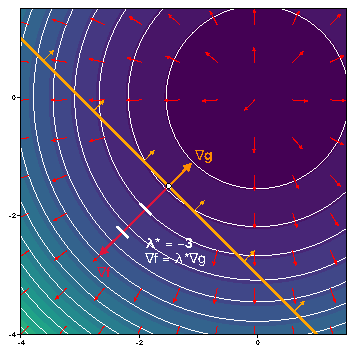
\includegraphics[width=0.8\textwidth]{../src/examples/constrained_optimum.pdf}
%\caption{Test}
%\label{eq:constrained_optim}
%\end{figure}
%
%By introducing more constraints to $c(\mathbf{x}) =0$, first order necessary conditions of optimality are stated%  \ref{eq:lagrange} 
%
%\begin{equation}
%\nabla J(\mathbf{x}) + \symbf{\lambda} \nabla c(\mathbf{x})= 0  \label{eq:first_order},
%\end{equation}
%\begin{equation}
%c(\mathbf{x})= 0.
%\end{equation}
%Point which satisfies this conditions is either optimum, minimum or saddle point
%$\lambda$ is  known as Lagrange multiplier,it is not some meaningless valuable that is be thrown away after finding the solution.  $\lambda$ can be thought of as a measure of importance of given constraint on the objective function $J(\mathbf{x})$,this concept is particularly useful for sensitivity analysis. Formally: $\lambda$ quantifies the sensitivity of the optimal cost to the constraint: $\frac{dJ^*}{d c(\mathbf{x})} = -\lambda$, where $\varepsilon$ is a small perturbation to $c(\mathbf{x}) = \varepsilon$. A large $|\lambda|$ means the constraint is strongly limiting the optimum, $\lambda = 0$ means the constraint is inactive and could be removed without affecting $J^*$, aaah i should make sure it is like this.
%
%
%\subsection{Inequality constrained optimization}
%
%Covered in section \ref{subsection:barrier_problem_formulation}.
%
%\chapter{Transcription}
%this chapter deal with the problem of transcribing the continuous optimal control problem into direct optimization problem, that is with discrete states and controls. The task boils down to integrating a function by evaluating it at discrete steps, this is called quadrature. The most commonly used quadratures for optimal control are Gauss-Legendre, Gauss-Radau and Gauss-Lobatto. Methods which are using these quadratures are called pseudospectral collocation methods. These methods are representing the integral of the function using polynomial, they are called collocation methods, because they work by forcing the derivation of the approximating polynomial to be equal to right hand side of the differential equation it is solving. Key aspect of these methods is that they can represent the solution to differential equation without error up to the degree of approximating polynomial. pridat toto s konstantou ktora big O little o...
%
%The approximating polynomials are constructing with roots of legendre, sometinh something lagrange polynomials
%DX = F(X,U)
%
%barycentric weights
%
%
%
%collocation point = derivation is equal to the differential equation
%boundary point = the constraints to tie two segment together are used for the solution
%
%gauss legendre points odnt contain any of the endpoint, the endpoints have to be constrained by extra addConstraint
%gauss legendre collocation
%N is in number of collocation points, order of approximating polynomial is then  for LG = 2N-1, for LGR = 2N-2, for LGL = 2N-3






%\part{My Party}
%
%
%\part{Your Party}
%
%\blindmathtrue
%
%\blinddocument
%
%\begin{table}
%\begin{ctucolortab}
%\begin{tabular}{cc}
%\bfseries Foo & \bfseries Bar \\\Midrule
%foo1 & bar1 \\
%foo2 & bar2
%\end{tabular}
%\end{ctucolortab}
%\caption{Foobar.}
%\label{tab:foobar}
%\end{table}
%
%\begin{figure}
%
\includegraphics[width=0.4\textwidth]{ctu_logo_black}
%\caption{Black logo of the CTU in Pragueueue.}
%\end{figure}
%
%\begin{figure}[!t]
%
\includegraphics[width=0.4\textwidth]{ctu_logo_blue}
%\caption{Blue logo of the CTU in Pragueueue.}
%\end{figure}   
%
%\chapter{Conclusions}
%
%\section{Test --- this is just a little test of something in the table of contents}
%
%\subsection{Yes, table of contents}
%
%\begin{theorem}\begin{enumerate} \item Bla \item Blo \end{enumerate} \end{theorem}
%
%
%Lorem ipsum dolor sit amet, consectetur adipiscing elit. Duis interdum facilisis urna, at tincidunt leo consectetur non. Maecenas bibendum mi vitae libero pharetra, ac ullamcorper nulla pellentesque. Sed sit amet massa nunc. Aenean placerat a est sodales sagittis. Quisque purus nibh, auctor ut consectetur at, suscipit non erat. Donec condimentum porttitor risus, vitae fringilla lectus tincidunt nec. Nulla leo quam, commodo eu ornare non, iaculis sed nulla. Duis gravida lacus quis purus sodales, vitae malesuada justo ultricies. Vestibulum nisl nulla, commodo non pellentesque a, fringilla a risus. Ut quis magna nulla. Mauris vitae ultricies ante, in consectetur justo. 
%
%\medskip
%
%\begin{proof}\begin{enumerate} \item[8] Bla \item Blo \end{enumerate} \end{proof}


\appendix

\printindex

\bibliographystyle{plain}
\bibliography{ctutest/ctutest}

\end{document}